%%% The main file. It contains definitions of basic parameters and includes all other parts.

%% Settings for single-side (simplex) printing
% Margins: left 40mm, right 25mm, top and bottom 25mm
% (but beware, LaTeX adds 1in implicitly)
\documentclass[12pt,a4paper]{report}
\setlength\textwidth{145mm}
\setlength\textheight{247mm}
\setlength\oddsidemargin{15mm}
\setlength\evensidemargin{15mm}
\setlength\topmargin{0mm}
\setlength\headsep{0mm}
\setlength\headheight{0mm}
% \openright makes the following text appear on a right-hand page
\let\openright=\clearpage

%% Settings for two-sided (duplex) printing
% \documentclass[12pt,a4paper,twoside,openright]{report}
% \setlength\textwidth{145mm}
% \setlength\textheight{247mm}
% \setlength\oddsidemargin{14.2mm}
% \setlength\evensidemargin{0mm}
% \setlength\topmargin{0mm}
% \setlength\headsep{0mm}
% \setlength\headheight{0mm}
% \let\openright=\cleardoublepage

%% Generate PDF/A-2u
\usepackage[a-2u]{pdfx}

%% Character encoding: usually latin2, cp1250 or utf8:
\usepackage[utf8]{inputenc}

%% Prefer Latin Modern fonts
\usepackage{lmodern}

%% Further useful packages (included in most LaTeX distributions)
\usepackage{amsmath}        % extensions for typesetting of math
\usepackage{amsfonts}       % math fonts
\usepackage{amsthm}         % theorems, definitions, etc.
\usepackage{bbding}         % various symbols (squares, asterisks, scissors, ...)
\usepackage{bm}             % boldface symbols (\bm)
\usepackage{graphicx}       % embedding of pictures
\usepackage{fancyvrb}       % improved verbatim environment
\usepackage{natbib}         % citation style AUTHOR (YEAR), or AUTHOR [NUMBER]
\usepackage[nottoc]{tocbibind} % makes sure that bibliography and the lists
			    % of figures/tables are included in the table
			    % of contents
\usepackage{dcolumn}        % improved alignment of table columns
\usepackage{booktabs}       % improved horizontal lines in tables
\usepackage{paralist}       % improved enumerate and itemize
\usepackage{float}			% enables figure placement enforcing

\usepackage{xcolor}
\definecolor{commnetsGreen}{RGB}{0,110,0}
\definecolor{blockGray}{gray}{0.9}

\usepackage{listings}		% listings
\lstset{
    tabsize=4,
    breaklines=true,
    basicstyle=\scriptsize,
    xleftmargin=20pt,
    xrightmargin=20pt,
    showstringspaces=false,
    commentstyle=\color{gray},
    keywordstyle=\color{blue},
    stringstyle=\color{commnetsGreen}}
\lstdefinelanguage{XML}{
	morestring=[b]",
  	morestring=[s]{>}{<},
	identifierstyle=\color{blue},
	stringstyle=\color{black},
	keywordstyle=\color{red},}
	
\newsavebox\resheadingbox
\newcommand{\codebox}[1]{%
	\begin{center}\sbox\resheadingbox{\colorbox{blockGray}{%
		\begin{minipage}{\dimexpr\textwidth-2\fboxsep\relax}
			\centering
			\strut\ttfamily#1\ttfamily\strut
		\end{minipage}%
	}}
	\dp\resheadingbox\dimexpr\dp\resheadingbox\relax
	\usebox\resheadingbox
	\end{center}
}
	
\renewcommand\lstlistlistingname{List of Listings}
%\usepackage[usenames]{xcolor}  % typesetting in color

%%% Basic information on the thesis

% Thesis title in English (exactly as in the formal assignment)
\def\ThesisTitle{	Interoperability of compiled PHP framework with .NET environment and package management}

% Author of the thesis
\def\ThesisAuthor{Filip Horký}

% Year when the thesis is submitted
\def\YearSubmitted{2019}

% Name of the department or institute, where the work was officially assigned
% (according to the Organizational Structure of MFF UK in English,
% or a full name of a department outside MFF)
\def\Department{Department of Software Engineering}

% Is it a department (katedra), or an institute (ústav)?
\def\DeptType{Department}

% Thesis supervisor: name, surname and titles
\def\Supervisor{Ing. Mgr. Robert Husák}

% Supervisor's department (again according to Organizational structure of MFF)
\def\SupervisorsDepartment{Department of Software Engineering}

% Study programme and specialization
\def\StudyProgramme{Computer Science}
\def\StudyBranch{Programming and Software Systems}

% An optional dedication: you can thank whomever you wish (your supervisor,
% consultant, a person who lent the software, etc.)
\def\Dedication{%
Foremost, I would like to thank my supervisor Ing. Mgr. Robert Husák for all his time and much advice in the course of this thesis. I want to offer thanks to Markéta Sauerová for hours of grammar and syntax consulting. I am also thankful to the whole Peachpie dev team, especially RNDr. Jakub Míšek, for their support and tips. Last but not least, I would like to express gratitude to my parents and family for their love and support.
}

% Abstract (recommended length around 80-200 words; this is not a copy of your thesis assignment!)
\def\Abstract{%
PHP language dominates the web development industry for a long time now. Each major PHP framework brings together large community and a solid codebase, providing features and tools that make the PHP web application development even simpler. Joining this vast world with .NET is an aim of Peachpie, PHP compiler to .NET. This provides means to use Symfony framework in .NET, yielding advantages for both PHP developers striving for more security and .NET programmers lacking third-party content. Doing so with plain Peachpie compiler, however, brings problem of actual usability of the features Symfony provides. Each project would require to recompile Symfony Components again and thus result in both time overhead and tedious manual configuration. This thesis shows it is possible to improve this process and enable intuitive usage of Symfony framework in .NET environment. It denotes utilities for semi-automatic compilation of Symfony Components into NuGet packages and migration of simple Symfony applications to .NET. Furthermore, it provides tools for additional interoperability between Twig and Razor template engines, and a set of examples of its actual usage.
}

% 3 to 5 keywords (recommended), each enclosed in curly braces
\def\Keywords{%
{C\#} {PHP} {ASP.NET} {PeachPie} {Symfony}
}

%% The hyperref package for clickable links in PDF and also for storing
%% metadata to PDF (including the table of contents).
%% Most settings are pre-set by the pdfx package.
\hypersetup{unicode}
\hypersetup{breaklinks=true}

% Definitions of macros (see description inside)
%%% This file contains definitions of various useful macros and environments %%%
%%% Please add more macros here instead of cluttering other files with them. %%%

%%% Minor tweaks of style

% These macros employ a little dirty trick to convince LaTeX to typeset
% chapter headings sanely, without lots of empty space above them.
% Feel free to ignore.
\makeatletter
\def\@makechapterhead#1{
  {\parindent \z@ \raggedright \normalfont
   \LARGE\bfseries \thechapter. #1
   \par\nobreak
   \vskip 20\p@
}}
\def\@makeschapterhead#1{
  {\parindent \z@ \raggedright \normalfont
   \LARGE\bfseries #1
   \par\nobreak
   \vskip 20\p@
}}
\makeatother

% This macro defines a chapter, which is not numbered, but is included
% in the table of contents.
\def\chapwithtoc#1{
\chapter*{#1}
\addcontentsline{toc}{chapter}{#1}
}

% Draw black "slugs" whenever a line overflows, so that we can spot it easily.
\overfullrule=1mm

%%% Macros for definitions, theorems, claims, examples, ... (requires amsthm package)

\theoremstyle{plain}
\newtheorem{thm}{Theorem}
\newtheorem{lemma}[thm]{Lemma}
\newtheorem{claim}[thm]{Claim}

\theoremstyle{plain}
\newtheorem{defn}{Definition}

\theoremstyle{remark}
\newtheorem*{cor}{Corollary}
\newtheorem*{rem}{Remark}
\newtheorem*{example}{Example}

%%% An environment for proofs

%%% FIXME %%% \newenvironment{proof}{
%%% FIXME %%%   \par\medskip\noindent
%%% FIXME %%%   \textit{Proof}.
%%% FIXME %%% }{
%%% FIXME %%% \newline
%%% FIXME %%% \rightline{$\square$}  % or \SquareCastShadowBottomRight from bbding package
%%% FIXME %%% }

%%% An environment for typesetting of program code and input/output
%%% of programs. (Requires the fancyvrb package -- fancy verbatim.)

\DefineVerbatimEnvironment{code}{Verbatim}{fontsize=\small, frame=single}

%%% The field of all real and natural numbers
\newcommand{\R}{\mathbb{R}}
\newcommand{\N}{\mathbb{N}}

%%% Useful operators for statistics and probability
\DeclareMathOperator{\pr}{\textsf{P}}
\DeclareMathOperator{\E}{\textsf{E}\,}
\DeclareMathOperator{\var}{\textrm{var}}
\DeclareMathOperator{\sd}{\textrm{sd}}

%%% Transposition of a vector/matrix
\newcommand{\T}[1]{#1^\top}

%%% Various math goodies
\newcommand{\goto}{\rightarrow}
\newcommand{\gotop}{\stackrel{P}{\longrightarrow}}
\newcommand{\maon}[1]{o(n^{#1})}
\newcommand{\abs}[1]{\left|{#1}\right|}
\newcommand{\dint}{\int_0^\tau\!\!\int_0^\tau}
\newcommand{\isqr}[1]{\frac{1}{\sqrt{#1}}}

%%% Various table goodies
\newcommand{\pulrad}[1]{\raisebox{1.5ex}[0pt]{#1}}
\newcommand{\mc}[1]{\multicolumn{1}{c}{#1}}


% Title page and various mandatory informational pages
\begin{document}
%%% Title page of the thesis and other mandatory pages

%%% Title page of the thesis

\pagestyle{empty}
\hypersetup{pageanchor=false}
\begin{center}

\centerline{\mbox{
\includegraphics[width=166mm]{img/logo-en.pdf}}}

\vspace{-8mm}
\vfill

{\bf\Large BACHELOR THESIS}

\vfill

{\LARGE\ThesisAuthor}

\vspace{15mm}

{\LARGE\bfseries\ThesisTitle}

\vfill

\Department

\vfill

\begin{tabular}{rl}

Supervisor of the bachelor thesis: & \Supervisor \\
\noalign{\vspace{2mm}}
Study programme: & \StudyProgramme \\
\noalign{\vspace{2mm}}
Study branch: & \StudyBranch \\
\end{tabular}

\vfill

% Zde doplňte rok
Prague \YearSubmitted

\end{center}

\newpage

%%% Here should be a bound sheet included -- a signed copy of the "bachelor
%%% thesis assignment". This assignment is NOT a part of the electronic
%%% version of the thesis. DO NOT SCAN.

%%% A page with a solemn declaration to the bachelor thesis

\openright
\hypersetup{pageanchor=true}
\pagestyle{plain}
\pagenumbering{roman}
\vglue 0pt plus 1fill

\noindent
I declare that I carried out this bachelor thesis independently, and only with the cited
sources, literature and other professional sources.

\medskip\noindent
I understand that my work relates to the rights and obligations under the Act No.~121/2000 Sb.,
the Copyright Act, as amended, in particular the fact that the Charles
University has the right to conclude a license agreement on the use of this
work as a school work pursuant to Section 60 subsection 1 of the Copyright Act.

\vspace{10mm}

\hbox{\hbox to 0.5\hsize{%
In ........ date ............	% FIXME!
\hss}\hbox to 0.5\hsize{%
signature of the author
\hss}}

\vspace{20mm}
\newpage

%%% Dedication

\openright

\noindent
\Dedication

\newpage

%%% Mandatory information page of the thesis

\openright

\vbox to 0.5\vsize{
\setlength\parindent{0mm}
\setlength\parskip{5mm}

Title:
\ThesisTitle

Author:
\ThesisAuthor

\DeptType:
\Department

Supervisor:
\Supervisor, \SupervisorsDepartment

Abstract:
\Abstract

Keywords:
\Keywords

\vss}

\newpage

\openright
\pagestyle{plain}
\pagenumbering{arabic}
\setcounter{page}{1}


%%% A page with automatically generated table of contents of the bachelor thesis

\setcounter{tocdepth}{1}
\tableofcontents

%%% Each chapter is kept in a separate file
\chapter*{Introduction}
\addcontentsline{toc}{chapter}{Introduction}

Speaking of programming languages, the present world of web development is divided into several nearly disjoint communities. Each of these communities focuses primarily on different aspect of development, for instance security, reliability or simplicity. However, the emphasized aspect of development is merely a consequence of the actual programming language selected for the implementation. Speaking of programming languages, we implicitly mean the server-side programming languages as the thesis is focuses mainly on them.

When it comes down to numbers, PHP: Hypertext Preprocessor (PHP) is the ultimate winner with the percentual usage between the websites surveyed of 60 to 70 \%. The second place holds ASP.NET with 10\% - 20\% usage. The third and fourth places are occupied by Java and Ruby, both situated around the border of 5 \% of usage \citep{w3techs.surveys, builwith.survey}. 

Previous statistics show that if we were to sum the websites implemented in PHP and .NET, we would end up with almost 80 \% of all surveyed, and presumably 8 out of 10 all existing, web applications. Moreover, unifying the two technologies would benefit both communities. Where the PHP community could make use of security and manageability advantages of pre-compiled code, the .NET developers will be given means to use dynamic features of the PHP language and a vast of community libraries. This is the ultimate goal of Peachpie, a modern PHP to .NET compiler, that is currently in development.

Many web oriented PHP frameworks have been developed by utilizing built-in functionalities of PHP such as response and request handling, and providing them in a more abstract way. This results in making the process of web application deployment faster and thus less expensive. Due to lack of any reliable statistics on the PHP web frameworks' usage, custom survey on the topic was performed. Considered parameters were Stack Overflow Trends, Google Trends, GitHub stars, Twitter followers and Facebook likes. This gives us quite accurate information about the popularity of selected frameworks compared to each other, which should at least correspond to their actual usage. Gathered data are displayed in the Figure 1 and apply to 15/04/2020. When evaluated, Wordpress is an absolute winner, followed by Laravel and Shopify that share the second place. Third place holds Symfony and after that comes the rest of compared frameworks such as CodeIgniter, PrestaShop, Zend or CakePHP.

Unfortunately, every web framework wraps PHP in its own unique way and provides special additional features. Some provide a basic functionality in a set of default scripts and a vast library of downloadable components with additional functionalities. Others deliver almost a working solution out of the box and leave the user only with the need to configure content and possibility to install whole features in a form of modules, such frameworks are usually called Content Management Systems or simply CMS. Therefore, each framework requires special treatment during its compilation, making their automatic compilation impossible. The Peachpie developers have successfully compiled Wordpress framework. Shopify is not open-source and thus its source code is not simply accessible. On the other hand, Laravel is open-source, and the same goes for Symfony. Even though Laravel is in popularity superior to Symfony, Symfony is almost twice as old and its packages are produced mostly by teams recognized by the Symfony developers themselves, for example FOS or KnpLabs can be named. Its long lasting stability and guaranteed quality of its packages has proved Symfony to be the perfect adept for compilation.

This work therefore examines the possibilities of compiling the Symfony framework into the .NET platform. However, the Peachpie compiler provides just the tools for a single PHP project into .NET compilation. This approach is unfortunate for the Symfony framework as its philosophy lays in minimal start-up project, where every secondary functionality is provided via additional libraries. Therefore, for the purpose of saving user's compilation and start-up time, those libraries are to be precompiled and supplied to projects in the quantity that they require, rather than to compile the project and all of its libraries for each project over and over again. For this task, The NuGet package manager has been selected as it shares the same ideology with Composer, a package manager that is tightly coupled with the Symfony framework. The ideology mentioned focuses mainly on package and dependency management at the project level. Besides, its wide spread of usage, Visual Studio integration ability and fairly easy usability were also taken into consideration.

\begin{figure}[h]
  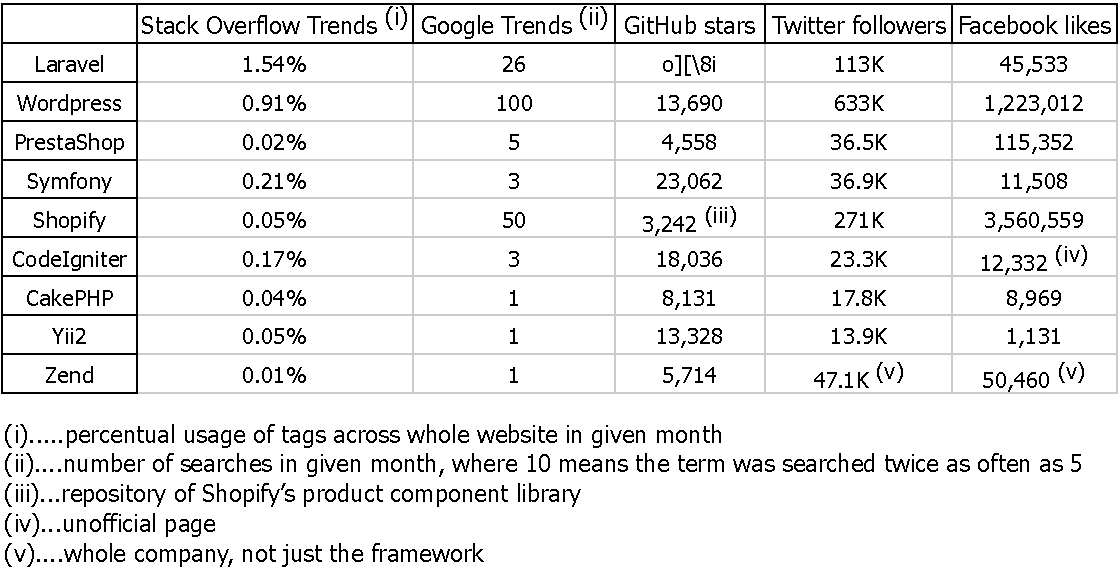
\includegraphics[width=\linewidth]{img/PHP_frameworks_popularity.pdf}
  \caption{PHP frameworks popularity comparison}
  \label{fig:php_frameworks_popularity}
\end{figure}


\section*{Thesis overview}
\addcontentsline{toc}{section}{An overview of the thesis}

The first chapter introduces the PHP programming language along with the tools like the Composer package manager, the Symfony framework and Twig template engine. The second chapter provides general overview of the C\# programming language and tools associated with it: NuGet package manager, ASP.NET Core and Razor template engine. Chapter 3 addresses the problematique of compiling one language to another in general and introduces Peachpie, the PHP to .NET compiler. The problem the thesis aims to resolve along with proposed solution and possible alternatives is introduced in Chapter 4. The fifth chapter focuses on the Symfony Components compilation and the tools that assist the process. The way Symfony projects are compiled and deployed is discussed in Chapter 6. Chapter 7 describes actual usage of the toolkit provided with two exemplar applications.

\chapter{PHP language}
PHP is a general-purpose scripting language. It originated as a collection of Common Gateway Interface (CGI) scripts, written in PERL by Rasmus Lerdorf \citep{modern.php}. CGI scipt is a program executed by a server upon a request, whose output is then returned to a client \citep{cgi.perl}. It is essentially what makes server more than a collection of static resources \citep{cgi.perl}. Soon after their release, these PERL scripts were rewritten in C programming language to enhance their performance \citep{modern.php}. Since then, the underlying parser has been rewritten several times and many people were involved in implementing additional features and support libraries for this language \citep{php.manual}. 

PHP has been developed solely by individuals joining their effort. It has resulted in an organic growth of the language in a community of developers. On the one hand, environment in which the language grew caused many useful features and functions to be included in its core \citep{php.manual}. On the other hand, lack of supervision and pre-planning has produced significant inconsistency in function names and in order of functional parameters \citep{php.manual}. Furthermore, for over 20 years, no formal language specification defining correct language syntax existed \citep{Oscon2014}. This role was substituted by PHP's engine and the ``If it works, then it's fine" philosophy \citep{Oscon2014}. This task was addressed in 2014 and the resulting document is being further extended since by both, PHP community and the PHP Group \citep{Oscon2014, php.spec}. The PHP group is a comunity of developers that maintain both, PHP language repository on github and php.net web portal with all the necessary information about the language, from news about releases to actual language documentation.

Versioning of the language might prove to be quite confusing as the official name "PHP" language holds since version 3.0 \citep{php.manual}. Version 1.0 was more of a set of CGI tools than an actual standalone language and version 6.0 was left abandoned due to insufficient number of contributors considering the amount of work that promised unicode support brought \citep{php.manual, php.version6}. PHP versioning officially uses the [major].[minor].[release] scheme, but as the releases of the same major and minor version differ mostly in the number of bugs fixed, only the [major].[minor] scheme is generally used. Currently, PHP 7.4 is the latest stable released version, therefore, when speaking of PHP language without explicit version number mentioning, PHP version 7.4 is meant.

\paragraph{Execution}
PHP is an interpreted scripting programming language. Although both terms can be defined in several different ways, for the purpose of this text, we understand these terms as that the language was designed for a special-runtime environment without the need to be compiled. PHP scripts are executed by the Zend Engine, an open-source set of components than provide PHP language with tools for its processing and execution \citep{php.internals, modern.php}. It was written in C programming language by Zeev Suraski and Andi Gutmans for PHP version 4, after their previous collaboration with Rasmus Lerdorf on PHP version 3 \citep{php.manual}. Since then, 2 new versions of Zend Engine has been introduced, each time bringing new major version of PHP language \citep{php.manual, php.wiki}.

\paragraph{The Zend Engine}
Undoubtedly, the most important component of the Zend Engine is the Zend Virtual Machine (VM), responsible for interpretation of PHP script \citep{php.internals}. The first step the Zend VM performs when executing a PHP script is a lexical analysis \citep{advanced.php}. There it converts human-readable code to tokens for further procession. The parser then takes the stream of tokens and generates an intermediate code \citep{advanced.php}. Code optimizations can be performed during this stage, including resolving simple function calls with literal arguments, constant mathematical expressions folding or unreachable code removing \citep{advanced.php}. This part of PHP script processing is called the compilation phase, preceding the execution phase \citep{advanced.php}. After that, intermediate code in a form of an ordered array of opcodes is passed to the executor that steps through the array and executes each instruction in turn \citep{advanced.php}. 

One of the main features of the Zend Engine is its extensibility \citep{advanced.php}. The engine supports modifications either by using Zend extension API or through alterable function pointers \citep{advanced.php}. For example, both \texttt{zend{\_}compile} and \texttt{zend{\_}execute} functions that handle script processing phases are implemented internally as function pointers, making it possible for further custom overloading of these functions at runtime \citep{advanced.php}. 

The process of PHP application's execution is also illustrated in the following Figure.

\begin{figure}[h]
  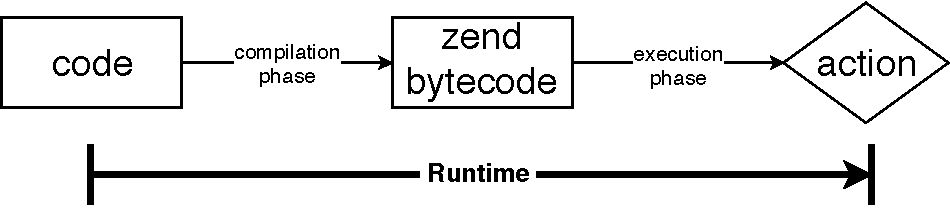
\includegraphics[width=\linewidth]{img/PHP.pdf}
  \caption{PHP's execution}
  \label{fig:php_execution}
\end{figure}





\section{Language features}
\paragraph{Object Oriented Programming}
Since the language version 5, Object Oriented Programming (OOP) is possible \citep{php.manual}. This enables developers to introduce another layer of abstraction above PHP code, possibly bringing higher level of organization and reducing maintenance burden. PHP supports all expected constructs of OOP such as Classes, Interfaces, Constructors and Inheritance \citep{php.manual}. On a class instantiation, \texttt{object} data type is created \citep{php.manual}. Every object is completely independent, holding its own properties and defined solely by a class it was instantiated from \citep{php.manual}. 

\paragraph{Type System}
PHP programming language is dynamically typed. This means that the language implicitly performs conversion between two types from different families, such as numbers and strings. This approach provides the language with additional flexibility and agility but does so at a cost of increased complexity and reduced safety. For instance, a developer with knowledge of how does inner conversion work is able to pass \texttt{integer 42} to a function expecting a \texttt{string} data type knowing, that the implicit conversion between the types will result in a \texttt{string 42}. On the other hand, an inexperienced developer might succeed comparing given variable with the equality operator \texttt{==} to \texttt{integer 42} without knowing that the variable actually holds \texttt{string 42}.

To decrease the required level of understanding of inner conversions and increase type safety, PHP provides several features for easier type manipulations and actively works on the development of the new ones. One of the most widely used amongst these features is the identity operator \texttt{===}, which extends the standard behaviour of equality operator with additional requirement for type equality of compared variables. Another much more recently added features are type hints, also called type declarations, and strict type checking \citep{php.manual}. These provide the means to specify both the expected types of function's parameters and its return type \citep{php.manual}. In case it is possible to perform an implicit conversion between the type provided and the type expected, the types declared in the function signature are by default for the purpose of backwards compatibility ignored \citep{php.manual}. However, strict type checking feature presents a way to force PHP interpreter to perform this additional type checking, enabling it to throw runtime errors on type mismatch, even when the implicit conversion is defined \citep{php.manual}.

Because of the dynamic nature of PHP data types, generic type relations are possible without any special constructs. However, this does only provide a way for a basic usage of generics in a form of what is in other languages called generic collections and generic function declarations. It does not allow for any further type relationships, such as bounding of generic types, to be declared and checked.

Special place between PHP data structures hold arrays. Internally, arrays are represented as ordered maps \citep{php.manual}. When provided, arrays use custom string or integer values as a keys for indexing, basic 0 based keys are used otherwise. Arrays with custom keys are called associative arrays. It is also notable that PHP does not throw an exception when float, boolean or null values are used as keys of an array \citep{php.manual}. Instead, as strings and integers are the only supported key types, implicit conversions between the types are performed \citep{php.manual}. On top of that, string keys representing a valid integer number are implicitly converted to integer keys \citep{php.manual}. 

\paragraph{Variables}
When a variable is declared by a standard syntactic mean of \$ sign followed by the case sensitive name of the variable, PHP disallows any explicit type definitions. Variable's type is determined by the context in which it is used, making it possible to seamlessly switch between types with a simple value assignment \citep{php.manual}. Moreover, PHP itself does not requite any formal declaration of variables \citep{php.manual}. The variable is automatically created the first time it is used in a scope and ceases to exist when it is set to null or \texttt{unset} method for this variable is called \citep{php.manual}. 

\paragraph{Request and Response}
As was mentioned before, PHP was designed to run on servers as a form of abstraction over the typical request-response based conversation between a client and a server. To abstract developers from actual HTTP request and to relieve them of the need for repetitive request parsing, several superglobal variables were built-in \citep{php.manual}. As the name suggests, these variables are always accessible, regardless the current scope. \texttt{\${\_}SERVER, \${\_}GET, \${\_}POST} and \texttt{\${\_}REQUEST} are all members of this group of variables. All of them contain parsed and ready to use data either about the request itself, such as uri or headers, or about data provided by the request, like submitted form fields and URL encoded parameters \citep{php.manual}.

Futhermore, PHP provides means to easily create HTTP response in just a few lines, taking care of the actual HTTP response creation itself. For instance the \texttt{header} function accepts a string as a parameter and setts it as one of returned response's headers \citep{php.manual}. Additionally, the most profound PHP construct \texttt{echo} is also used in this context as it takes its parameters and appends them to the response's body \citep{php.manual}. 



\section{Composer}
Composer is a tool for managing dependencies in PHP. Composer works with libraries, sometimes referred to as packages or projects, on a per-project basis. This is what differs the tool from traditional Linux package managers such as APT as they usually install packages globally, for computer's operating system, making it more similar to NPM or YARN managers \citep{composer.docs}. These libraries composer works with are zip archives of \texttt{composer.json} configuration file, code, optional \texttt{composer.lock} file and any other code-related resources \citep{composer.docs}.

When composer executes a command, in most cases either input or output of the command is a \texttt{composer.json} configuration file or its update. This file provides means to specify basic information about the package like its name, description, dependencies or type, which can be of project, library, metapackage or composer-plugin \citep{composer.docs}. It can be also used to specify additional package repositories and to define scripts as aliases of command-line executables whose execution can be linked to composer's commands \citep{composer.docs}. Where some commands, like \texttt{install} or \texttt{update}, do require the \texttt{composer.json} file's existence prior to their execution, as their functionality lays in loading current package's configuration and acting upon it, other commands, such as \texttt{require} or \texttt{create-project}, only settle for their arguments and the \texttt{composer.json} file's creation or modification is a result of their work \citep{composer.docs}.

Third-party libraries installation is done via require command suffixed with library's name and an optional version number \citep{composer.docs}. When resolving a package, one possible outcome is composer finding a zip archive of this library, in which case its contents is unzipped to a \texttt{vendor/[libraryName]} folder \citep{composer.docs}. Sometimes a metapackage is found instead. These are empty packages containing just a composer.json file with basic information and a list of dependencies and a \texttt{readme.md}, as they are usually hosted on version control services \citep{composer.docs}. In this case, new instance of composer is created for this \texttt{composer.json} configuration file and installation of listed dependencies is triggered. Both ways result in one or more added libraries to vendor directory. Every package installation or update also result in either update or creation of a \texttt{composer.lock} file. Where \texttt{composer.json} file holds a list of packages and basic information about current project, the \texttt{composer.lock} file notes actual version of each package resolved by the composer and can be therefore used to ensure that the same set of dependencies is installed in all the instances of the project. 





\section{Symfony framework}
Symfony is a PHP framework for web application development. It is built on top of the Symfony Components, a set of reusable PHP libraries \citep{symfony.reference}. Each library provides certain functionalities and many of them are completely independent, making it possible to use them without the need for using the Symfony framework itself \citep{symfony.reference}. This universality gave birth to many new web frameworks such as Laravel or Drupal version 8, which are built atop the Symfony Components as well \citep{symfony.reference}.

The Symfony framework evolves a lot each time a major version is released but its philosophy remains. It is to give developers full control over the project's configuration, from the directory structure to a set of used libraries \citep{symfony.reference}. When the work on the project began, Symfony 4.2 was the latest stable version of the framework released, for this reason, further description would primarily focus on this version.


\paragraph{Installation}
Bare bones Symfony application is created via composer, more precisely the \texttt{create-project} command with either the \texttt{symfony/website-skeleton} or the \texttt{Symfony/skeleton} argument \citep{symfony.reference}. When executed, composer downloads predefined set of core libraries that handle base framework functionality \citep{symfony.reference}. After that, everything from routing set-up to additional libraries downloading with the \texttt{composer require} command is up to developer.


\paragraph{Request and Response}
Symfony's way of request-response conversation handling is nothing more than an object-oriented abstraction of the PHP's one \citep{symfony.reference}. For this purpose, the \texttt{Request} and the \texttt{Response} classes, with specialized functions for request and response manipulation were introduced \citep{symfony.reference}. These two classes are part of a Symfony Component called \texttt{symfony/http-foundation}, which is included by composer on application's skeleton installation \citep{symfony.reference}.

\paragraph{Front Controller}
Traditional small PHP applications usually follow a simple pattern, where each site's page is represented by a physical file, for example \texttt{index.php}. As the size of an application increases, this approach brings an overhead in the form of code repetition, complicated route changing and overall decreased flexibility. For this purpose, larger application may define single PHP script called Front Controller, that handles every incoming request and calls another, more specialized controllers that provide actual response \citep{advanced.php}. 

The Symfony framework is no exception to this approach. However, instead of specialized controller calling, everything Symfony's front controller does is booting Symfony and passing information about the request \citep{symfony.reference}. This is done by executing the \texttt{src\textbackslash{}Kernel.php} script \citep{symfony.reference}. Afterwards, \texttt{Kernel.php} uses the Routing component to interpret the request and to resolve the appropriate controller to be called \citep{symfony.reference}. Finally, based on request's method and parameters, selected function from the controller is executed, resulting in the Response object, that is converted by the Symfony framework to the HTTP response and sent back to the client \citep{symfony.reference}.




\section{Twig}
TWIG is a PHP library used to combine template files with data model to produce HTML documents. In other words, it is a template engine. Its syntax consists of HTML extended with TWIG code and three special delimiters. 

\paragraph{Output delimiter}
The first one is \texttt{\string{\string{...\string}\string}}, which is used for outputting results of expressions \citep{twig.docs}. These can be either variable names or function calls \citep{twig.docs}. TWIG has a small set of predefined functions \citep{twig.docs}. Some have straightforward functionality and self-explaining name such as dump and max, where other are much more complex, like include, resulting in included TWIG template loading, generating and embedding the result in the current template \citep{twig.docs}. Every expression can be suffixed with arbitrary number of \texttt{|[filterName]} expressions to further process result before its outputting \citep{twig.docs}. TWIG comes with approximately 40 filters such as upper, split and replace \citep{twig.docs}. The predefined filters and functions usually cover the basic usage of the engine. However, extending built-in functions and filters is also possible by writing PHP script extending the \texttt{AbstractExtension} class and defining the \texttt{getFilters} or the \texttt{getFunctions} method, which is used to link the filter's or the function's implementation method to its alias through which it can be further used \citep{twig.docs}. 

\paragraph{Other delimiters}
The second delimiter is \texttt{\string{\%...\%\string}}, used for executing statements and controlling the flow of a program \citep{twig.docs}. Supported structures are for instance \texttt{\string{\% for - in - \%\string}...\string{\% endfor \%\string}}, \texttt{\string{\% if - \%\string}...\string{\% endif \%\string}} or \texttt{\string{\% set - = - \%\string}} \citep{twig.docs}. Finally, comments are supported via the \texttt{\string{\# ... \#\string}} syntax \citep{twig.docs}.


\paragraph{Template inheritance}
The most useful and powerful feature of TWIG is template inheritance. This allows to build a template acting as a basis that child templates further extend. Such template may contain all the common elements of a site - header, footer and a navigation bar. Furthermore, it can define blocks with \texttt{\string{\% block - \%\string}...\string{\% endblock \%\string}} syntax, whose content can be either fully overwritten by child templates or combined with child's one via \texttt{\string{\string{ parent() \string}\string}} function \citep{twig.docs}. Inheritance is enabled for selected templates by specifying a parent template with \texttt{\string{\% extends - \%\string}} construct in the beginning of each child template \citep{twig.docs}.

\paragraph{Environment}
Environment is a object used for storing the configuration with possible extensions, loading and rendering of a template \citep{twig.docs}. The lookup and loading of a template is performed by a loader, class implementing the \texttt{\textbackslash{}Twig\textbackslash{}Loader\textbackslash{}LoaderInterface} interface, which is provided as a first parameter to the \texttt{\textbackslash{}Twig\textbackslash{}Environment} class constructor \citep{twig.docs}. Template is loaded with the \texttt{load} method of the Environment class and rendered with the \texttt{render} method of the \texttt{\textbackslash{}Twig\textbackslash{}TemplateWrapper} class, whose instance is returned by the load method \citep{twig.docs}. The \texttt{render} method takes either one parameter - an associative array of variable names and values that are to be provided to rendered template, in which case it acts as described before, or two parameters - template name and an array \citep{twig.docs}. The second form wraps both the loading and the rendering of the template internally, returning directly a rendered string of HTML markup \citep{twig.docs}. The \texttt{templateWrapper} class also provides a self-explanatory method \texttt{renderBlock} \citep{twig.docs}.

\paragraph{} A simple example of Twig template providing a header for calendar table is provided in the following Listing.

\begin{center}
\lstset{language=XML,
	morekeywords={colspan, class, title}}
\begin{lstlisting}[caption={Twig example},captionpos=b]
<thead>
	<tr>
		<th colspan="7" class="month">
			{{ monthnames[month].full }}
        </th>
    </tr>
    <tr>
        {% for dow in range(0, 6) %}
        	{% set day = (dow + firstDay) % 7 %}
            <th class="
            	day {% if (day == 6 or day == 0) %}weekend{% endif %}
            ">
            	<span title="{{ daynames[day].full }}">
            		{{ daynames[day].short }}
            	</span>
            </th>
       {% endfor %}
	</tr>
</thead>
\end{lstlisting}
\end{center}


\chapter{C\# language}
The goal of this chapter is to introduce C\# programming language and .NET platform. The following part of the chapter will focus on NuGet package manager as it forms a building block for the upcoming text. Furthermore, ASP.NET Core framework's background will be described, accompanied by an introduction to Razor markup, which is tightly entangled with ASP.NET Core. Both the ASP.NET Core part and the Razor part will also present an overview of their usage with simple code examples.

\section{Language introduction}
C\# is a general-purpose programming language, under the management of Microsoft Corporation. It is a part of the developer platform called .NET. One of the main features of .NET is language interoperability, giving programmer opportunity to combine multiple languages and libraries in a single project. That is possible because of the same specification that all .NET components are build atop, called the Common Language Infrastructure (CLI) \citep{Ecma335}. The CLI has been standardized by ECMA International in ECMA-335 and approved as ISO/IEC 23271 \citep{Ecma335}. This document covers following 4 areas of interest: type system, metadata, the Common Language Specification (CLS) and the Virtual Execution System (VES) \citep{Ecma335}. 

At the time of writing, there are 8 major versions of C\# programming language released \citep{microsoft.docs}. When speaking of C\# we implicitly mean C\# version 8, as the latest officially released version.

\paragraph{Type system}
The question of types and their definitions is answered by the Common Type System (CTS) \citep{Ecma335}. In order to cover type systems of wide range of programming languages, the CTS defines large number of types and operations \citep{Ecma335}. 

\paragraph{Metadata}
\textit{"Metadata are used as a way to describe and reference the types defined by the CTS. For that purpose, they are stored in a way that is independent of any particular programming language"} \citep{Ecma335}.

\paragraph{Assemblies}
With language-unique compilers, each .NET project is compiled to the Common Intermediate Language (CIL), also known as managed code or simply IL \citep{Ecma335, ProCSharp}. Resulted compiled code is then saved as either a Dynamically Linked Library (DLL) or en Executable file (EXE) \citep{ProCSharp}. Basically, when the compiled code specifies the application's entry point, EXE file is generated, DLL file is generated otherwise \citep{ProCSharp}. Exception to this behaviour brought .NET Core, which makes it possible to generate DLL files for both, code with and without an entry point \citep{microsoft.docs}. Generated DLLs and EXEs together are called assemblies \citep{ProCSharp}.

\paragraph{The Common Language Specification}
The CLS specifies a subset of the CTS and a set of rules that publicly exported aspects of compiled assemblies shall follow in order to ensure language interoperability \citep{Ecma335}. Its aim is to provide developers with the same base types and usage conventions for each framework that adhere the CLS. \citep{Ecma335}

\paragraph{Virtual Execution System}
The VES is responsible for loading and running programs written for the CTS \citep{Ecma335}. It provides the services needed to execute managed code and data, using the metadata to connect separately generated modules together at runtime (late binding) \citep{Ecma335}. On runtime, platform-specific implementation of the VES performs just-in-time (JIT) compilation of the CIL code to the native code \citep{Ecma335}.

\paragraph{.NET Standard}
In addition to the CLI, .NET Standard was introduced as a way to establish greater uniformity in the .NET environment \citep{ProCSharp}. In contrary to the CLI, .NET Standard only specifies a set of .NET APIs that are intended to be available on all .NET implementations \citep{microsoft.docs}. Each version of major .NET implementation, such as .NET Core, .NET Framework or Mono, targets specific versions of .NET Standard \citep{microsoft.docs}. Each application can target a version of a specific .NET implementation or version of .NET Standard, making it possible to run on any .NET implementation which supports that version of the .NET Standard \citep{ProCSharp}.

\paragraph{}
The process of C\# application's deployment from compilation to execution is summed up in the following Figure.

\begin{figure}[h]
  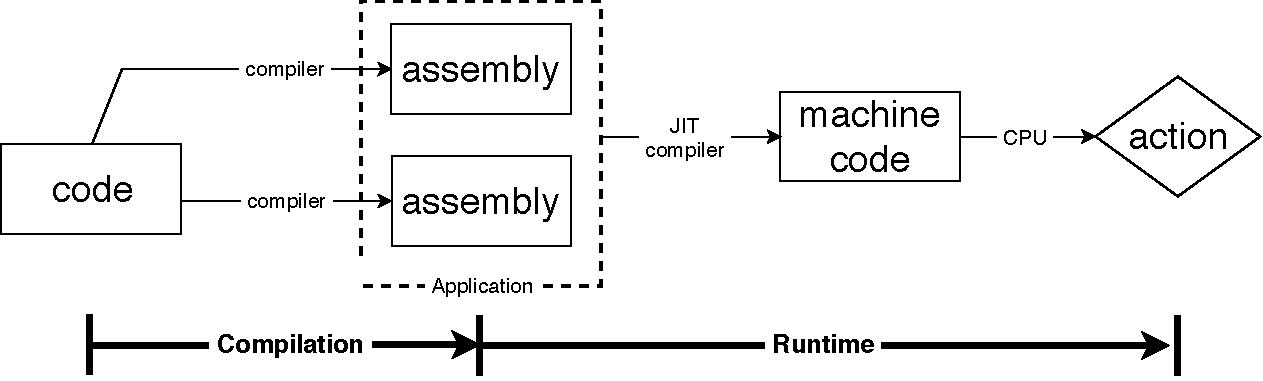
\includegraphics[width=\linewidth]{img/Csharp.pdf}
  \caption{C\# application's deployment}
  \label{fig:csharp_execution}
\end{figure}


\section{Language features}

\paragraph{Type system}
Types in C\# are divided into two main categories, value types and reference types. In contrary to value types, that directly hold their data, reference types hold only references to objects. There is also a type called \texttt{System.Object}. It is the base class of all types in C\#, meaning that every type in C\# can be converted to an object type (boxing) and vice versa (unboxing) \citep{microsoft.docs}. Because of that, the type system of C\# can be label as a Unified Type System. 

Slightly aside from this, stands the dynamic type. Its features are, in terms of boxing and unboxing, very close to those of base object type \citep{microsoft.docs}. The point where dynamic type differs from base object type is in the amount of information compiler has about the type, and in the way type is processed on runtime \citep{microsoft.docs}. An example illustrating both those differences is casting \citep{microsoft.docs}. Dynamic variables do not require any explicit type casting, fully relying on the programmers' knowledge of what he or she is doing \citep{microsoft.docs}. Main purpose of dynamic types is to allow interactions with dynamic objects, such as objects from other programming languages with type systems different than the one of C\# \citep{microsoft.docs}.

\paragraph{Variables}
In C\#, every variable has a type that determines what values can be stored in the variable \citep{microsoft.docs}. On compilation, C\# compiler validates whether each value stored in a variable is of the appropriate type and whether there are no operations with given variable, that are invalid for its type \citep{microsoft.docs}. In other words, C\# is type safe.

There is also requirement for each variable to be definitely assigned before C\# compiler allows for its value to be obtained \citep{microsoft.docs}. Microsoft documentation defines definitely assigned variable as follows: \textit{"At a given location in the executable code of a function member, a variable is said to be definitely assigned if the compiler can prove, by a particular static flow analysis, that the variable has been automatically initialized or has been the target of at least one assignment"} \citep{microsoft.docs}. 


\section{NuGet}
NuGet is Microsoft-supported mechanism for creating, sharing and consuming code under the .NET environment \citep{microsoft.docs}. For this purpose NuGet defines a \texttt{package}, single unit of compiled code, related resources and a descriptive manifest containing necessary information about both, the package and the code it holds \citep{microsoft.docs}. These packages are generally nothing more than a \texttt{.zip} archive of mentioned three groups of files with \texttt{.nupkg} extension \citep{microsoft.docs}. 

In order to allow other developers to download and use a package, when created, a package is usually published to some kind of a sharing service \citep{microsoft.docs}. Depending on desired accessibility level, it can be publicly accessible hosting service such as \texttt{nuget.org}, a cloud, a network or a local file system \citep{microsoft.docs}.

Prior to a package usage, one must first ensure that the package and its required version has been installed \citep{microsoft.docs}. Regardless the method used for the package installation, NuGet always merges \texttt{packageSources} from \texttt{NuGetDefaults.config} file with any other \texttt{Nuget.config} files found and retrieves desired package using resulting collection \citep{microsoft.docs}. After that, content of \texttt{.nupkg} archive is simply copied to user-specific package folder \citep{microsoft.docs}. Finally, project files are updated and any missing package dependencies are installed \citep{microsoft.docs}. 




\section{ASP.NET Core}
ASP.NET Core is a framework focused on building web applications, based on .NET Core \citep{microsoft.docs}. Fundamentals of ASP.NET Core lies in request raising and handling \citep{microsoft.docs}. Every web application defines a pipeline that each component uses for its requests publishing \citep{microsoft.docs}. This pipeline composes of series of middleware components, placed in the order regarding the order of their request processing \citep{microsoft.docs}. When request is processed, each middleware component performs an asynchronous operation on \texttt{HttpContext} and decides, whether to invoke the next middleware component in the pipeline or to terminate the request by short-circuiting the pipeline \citep{microsoft.docs}.

\paragraph{Host}
One Layer above the pipeline stands the \texttt{Host} object \citep{microsoft.docs}. Its purpose is to encapsulate a HTTP server implementation, middleware components, logging, dependency injection and configuration by a single object, in order to simplify application start up and shut down control \citep{microsoft.docs}. ASP.NET Core provides the \texttt{WebHost} class with \texttt{CreateDefaultBuilder} method to set up a host with commonly used options, making most of the hard job in developer's stead \citep{microsoft.docs}.

Example of the \texttt{Host} object configuration and execution is provided by the following Listing.

\begin{center}
\lstset{language=[Sharp]C,
	morekeywords={var}}
\begin{lstlisting}[caption={Startup.Configure method},captionpos=b]
static void Main(string[] args)
{
	var host = WebHost.CreateDefaultBuilder(args)
					  .UseStartup<Startup>()
					  .UseUrls("http://*:5004/")
					  .Build();

	host.Run();
}
\end{lstlisting}
\end{center}

\paragraph{Middleware}
Mentioned middleware component, also called request delegate, can be one of built-in components or custom one \citep{microsoft.docs}. Each component is added to the pipeline in \texttt{Startup.Configure} method by invoking its \texttt{Use}, \texttt{Run} or \texttt{Map} extension method \citep{microsoft.docs}. By convention, \texttt{Use[middlewareName]} method decides whether to invoke the next middleware component in the pipeline \citep{microsoft.docs}. \texttt{Run[middlewareName]} methods runs at the end of the pipeline, terminating the pipeline after its processing \citep{microsoft.docs}. Finally, \texttt{Map[middlewareName]} method is used for branching the pipeline based on the matches of the given request path \citep{microsoft.docs}.

Following Listing displays one possible \texttt{Startup.Configure} method appearance. Such configuration adds the SessionMiddleware to enable session state for the application \citep{microsoft.docs}. The \texttt{UsePhp} method is extension of Kestrel provided by PeachPie software and will be spoken of later. Remaining \texttt{UseDefaultFiles} and \texttt{UseStaticFiles} handle file mappings and static file serving \citep{microsoft.docs}.
\begin{center}
\lstset{language=[Sharp]C}
\begin{lstlisting}[caption={Startup.Configure method},captionpos=b]
public void Configure(IApplicationBuilder app)
{
	app.UseSession();
	app.UsePhp(new PhpRequestOptions(scriptAssemblyName: "pageName"));
	app.UseDefaultFiles();
	app.UseStaticFiles();
}
\end{lstlisting}
\end{center}

\paragraph{UseMvc method}
The \texttt{UseMvc} extension method adds routing middleware to the request pipeline and configures Mvc as the default handler \citep{microsoft.docs}. ASP.NET Core MVC is a rich framework for building web apps and APIs using the Model-View-Controller design pattern \citep{microsoft.docs}.

Concept of the Model-View-Controller pattern lays in separation of application logic into three parts, kept in different folders, connected together via naming conventions \citep{microsoft.docs}. The model, representing the state of the application, usually holds data, performs user actions and retrieves results of queries \citep{microsoft.docs}. The View is a Razor template, responsible for a user interface building and content presenting \citep{microsoft.docs}. The Controller's job is selecting the view that is to be rendered in the response to the given request \citep{microsoft.docs}. This request can be either initial entry of given route or an user interaction \citep{microsoft.docs}. Additionally, it also provides chosen view with necessary information from the model \citep{microsoft.docs}. 

Given controller can be mapped to a route by calling the \texttt{MapRoute} extension method of routes object with targeted controller, its action (method) and possible suffix, all following the default conventional route syntax \citep{microsoft.docs}. Routing middleware also defines attribute routing, which allows for route definitions to be placed next to the controllers and actions which they are associated with \citep{microsoft.docs}. 

\paragraph{Services}
In ASP.NET Core, services are preregistered classes used by the application \citep{microsoft.docs}. User-defined services are registered in the \texttt{Startup.ConfigureServices} method \citep{microsoft.docs}. New classes can be registered as services to the \texttt{IServiceCollection} provided as a parameter to the function to be further available along with predefined framework-provided services \citep{microsoft.docs}. There is also a possibility to directly instantiate a service without the need for previous registration, using \texttt{ActivatorUtilities} \citep{microsoft.docs}.

By convention, each service is registered by calling the \texttt{Add[serviceName]} extension method of the \texttt{IServiceCollection} \citep{microsoft.docs}. When a service is registered, it is expected that both its configuration and its dependencies will be resolved, resulting in registration of all required services \citep{microsoft.docs}. This process is called the Dependency Injection (DI) and it is a practise from a design pattern with a same name.

Example of the \texttt{Startup.ConfigureServices} method is provided by the following Listing. It demonstrates a minimal configuration for project using just the distributed cache serviceand the session service.
\begin{center}
\lstset{language=[Sharp]C}
\begin{lstlisting}[caption={Startup.ConfigureServices method},captionpos=b]
public void ConfigureServices(IServiceCollection services)
{
	// Adds a default in-memory implementation of IDistributedCache.
	services.AddDistributedMemoryCache();

	services.AddSession(options =>
	{
		options.IdleTimeout = TimeSpan.FromMinutes(30);
		options.Cookie.HttpOnly = true;
	});
}
\end{lstlisting}
\end{center}





\section{Razor}
Razor is programming syntax used to create dynamic web pages through embedding server-generated code into websites \citep{microsoft.docs}. Its syntax consists of Razor markup, C\# and HTML \citep{microsoft.docs}.

HTML rendering is controlled via @ symbol. This symbol tells Razor to evaluate following C\# code, and optionally to render it in the HTML output \citep{microsoft.docs}. Rendered C\# code can be either single space-less expression, called implicit expression, or spaces supporting explicit expression \citep{microsoft.docs}. Implicit expressions are created as @ symbol directly followed by single space-less C\# statement, usually returning desired output \citep{microsoft.docs}. Explicit expressions can consist of several C\# statements, combining their outputs into result \citep{microsoft.docs}. These expressions are built using the \texttt{@(...)} pattern, where all the code inside the round brackets is processed as an explicit expression \citep{microsoft.docs}. Non-rendered C\# code uses pattern \texttt{@\string{...\string}} and can be further transformed into control structures, such as\texttt{@for(-;-;-)\string{...\string}}, \texttt{@switch(-)\string{...\string}} or \texttt{@using (-)\string{...\string}} \citep{microsoft.docs}. This block can also allow parts of its content to be rendered by @ symbol, @: directive or \texttt{<text>} tag \citep{microsoft.docs}.

In order to follow the DRY (Don't Repeat Yourself) principle, Razor introduced the Layout property. By specifying name or a full path of required layout file to be used, we tell the Razor rendering engine to encapsulate rendered content of current file with content of given layout file \citep{microsoft.docs}. This generated content is put in a place of the \texttt{RenderBody} method call inside a layout file \citep{microsoft.docs}. Additionally, custom sections can be defined in Razor views and Razor pages using the \texttt{@section} directive and rendered in layout files using the \texttt{@RenderSection} \citep{microsoft.docs}. This provides a way of additional code organizing \citep{microsoft.docs}. 

\paragraph{Razor View}
Razor Views are \texttt{.cshtml} files rendered by MVC controllers \citep{microsoft.docs}. Views associated with controllers are grouped in the folders named after them, in the Views folder at the root of the application \citep{microsoft.docs}. Additionally, view can correspond to a specific action, in which case, it is to be named after it \citep{microsoft.docs}. This arrangement makes application build with Razor views significantly easier to maintain, making it possible to build and update the application's views without necessity to update other parts of the application \citep{microsoft.docs}. It also contributes to testability and code reusability.

Process responsible for determining which view file is used is called view discovery \citep{microsoft.docs}. Actions initiate this process through calling public \texttt{View} method \citep{microsoft.docs}. By default, it searches folders \texttt{Views/[ControllerName]} and \texttt{Views/Shared} for view with the same name as the action method from which it is called \citep{microsoft.docs}. This behaviour can be changed by specifying a name or a file path of the view \citep{microsoft.docs}. 

\paragraph{Razor Page}
Besides the \texttt{UseMvc} method, Razor pages require additional services to be registered in \texttt{Startup.ConfigureServices} by calling either the \texttt{AddMvc} or the \texttt{AddMvcCore} extension method of the \texttt{IServiceCollection} \citep{microsoft.docs}.

The main difference between a Razor view and a Razor page lays in a controller \citep{microsoft.docs}. Razor page handles requests directly, without the need for going through a controller \citep{microsoft.docs}. For Razor pages, new directive \texttt{@page} has been introduced to distinguish in other aspects similar page files from view files \citep{microsoft.docs}. In all Razor pages, \texttt{@page} must be the first used directive \citep{microsoft.docs}. All razor pages are located in the Pages folder at the application root \citep{microsoft.docs}. This folder is also used as root for associations of URL paths to pages, as they are determined by the \texttt{.cshtml} file location on the file system, relative to the Pages folder \citep{microsoft.docs}.

Pages can be connected with the \texttt{PageModel} classes via the \texttt{@model [pageModelName]} directive \citep{microsoft.docs}. In this case, \texttt{PageModel} should be located in the same folder as the page file and its name should be created from the page's name by appending \texttt{.cs} suffix \citep{microsoft.docs}.

\paragraph{} A simple example of Razor template providing a header for calendar is in the following Listing.

\begin{center}
\lstset{language=XML,
	morekeywords={class}}
\begin{lstlisting}[caption={Razor example},captionpos=b]
<p class="month">
	@currentMonth - @current.Year
</p>
@for (int i = 0; i < 7; i++) {
	if (i == 0 || i == 6) {
		@:<div class="box_short weekend">
	} else {
		@:<div class="box_short">
	}
		@:@dayNames[i]
	</div>
}
\end{lstlisting}
\end{center}

\chapter{PHP to .NET compilation}
The third chapter talks about programming languages and communities around them in general. It provides a possible way of building a bridge between two selected communities and outlines some aspects of its practical implementation. Peachpie, an actual implementation of previously discussed tool is presented.

\section{Motivation}
In the recent days, web development, and software development in general, has evolved by a great bit in both the number of people involved and in a size of code produced. Web pages and applications are no longer just a several thousands of lines of code. For instance Facebook, one of the most profound social networks in the world, has a codebase of over 50 millions of lines of code \citep{Knowledge}. Moreover, it's not unusual for a codebase of software of an average modern high-end car to reach a hundred million lines of code \citep{Knowledge}. 

Natural consequence of such technological growth is that it is no longer possible to develop complex software alone and almost everything requires teaming up. Above the project-related groups of developers stands a community, where knowledge is shared and people learn from each other. While some patterns and practices are applicable in general, with increasing complexity of problem their amount is smaller and their usefulness decreases. This need for more definite knowledge has caused the community to be rather granulated and the number of breaching criteria is immense. Undoubtedly the most commonly used criteria is the one of programming languages.

A reasonable effort is put into attempts to bring together selected language-level sub-communities. Going through all of the possible methods of achieving this, is beyond the scope of the theses, so we will simply pick the one that is further relevant, the compilation method. It is worth mentioning that for this compilation method we require the target language to be an interpreted language. It is not to be misunderstood with method of compiling the second language to the source code of the target language, which would in that case be called the transcompilation method. Simply speaking, our compilation method means that we have a language A compiling into an interpreted language that is later executed. Then we take a language B and compile it with special tool into the same intermediate language as the language A. This allows us to embed parts of code from language B within our application written in language A. When this approach does not literally merge the sub-communities of languages A and B, it clearly provides a bridge between the two in a way of using features, knowledge and finally the developers of both languages in a single project \citep{Peachpie}.

For later usage, we would require a target language to be a compiled language with an efficient way to execute compiled code separated into multiple files. As was mentioned before, C\# is a compiled language with strictly defined foundation \citep{microsoft.docs}. In addition to, it has quite intuitive Integrated Development Environment (IDE) provided by Microsoft Corporation with many built-in features such as profiler and web designer \citep{microsoft.docs}. Finally, its assembly system allows for splitting application code between multiple files and their later efficient combination on runtime. For these reasons it is a perfect target for a compilation. On the other hand, PHP is an interpreted language with a large community of developers, many implemented libraries and vastly popular frameworks. Making it a possible candidate for a compilation.




\section{Languages comparison}
In programming generally, it is fairly unusual for two programming languages to share all, the same philosophy, capabilities and area of usage. When a problem in a certain language is encountered, solutions in other languages are mostly useless. This is addressed by a compilation method introduced before. When we encounter a problem in one language, have the solution in another language and ultimately have the means of compiling one language to another, the former solution quickly comes in hand. The crucial spot in the process are mentioned means for achieving the compilation. Prior to learning how to operate with the compiler tool, we first need to compare our candidates for the source and the target language. That is necessary in order to prepare for possible complications that might occur during the actual compilation.


\paragraph{Type System}
Even though there are significant differences in languages' type systems - one is statically typed, where the other one is dynamically typed, this difference will introduce no noticeable difficulties. PHP's engine is using types internally and those basic types are subset of the CTS \citep{php.internals, Ecma335}. In addition to, PHP has no sense of topology in its type system \citep{php.manual}. The types simply exist without any base types or inherited functions \citep{php.manual}. This makes their mapping to the .NET types and into its type hierarchy rather easy.

The only type-related complication is PHP's implicit conversion between the types. However, this problem can be solved easily by adding explicit conversions, implementing special functions that emulate PHP's implicit conversions between the types or for the sake of expensiveness using base type \texttt{Object} \citep{Phalanger}.


\paragraph{Variables}
As we already know, PHP does require type-less variable initialization whereas C\# requires explicit type definition when a new variable is initialized. Furthermore, PHP needs no variable initialization at all. On the contrary, C\#  presents a rule for each variable usage called the definitive assignment.

The problem of PHP's type-less initialization can be easily solved using implicit conversions mentioned in preceding paragraph and C\#'s base class \texttt{Object} \citep{Phalanger}. The problem of definitive assignment and PHP's ability to define variables in-place can be addressed on compilation \citep{Peachpie}. Based on each variable's usage, and for the sake of definitive assignment it can be simply initialized to null if needed. This operation will satisfy C\#'s variable requirements and will not divert from the behaviour observed in PHP, where uninitialized variables return null upon reading.


\paragraph{Execution}
One of the main differences between C\# and PHP lays in their execution. PHP is interpreted language whereas C\# is compiled. Although this difference in a deployment process might seem problematic, it is actually in our favour. If we were attempting to compile C\# to PHP, this might not be true as regarding PHP application's execution, such process would require compiler to transform C\# code to native PHP code.

On the other hand, in out case, we want to compile code of interpreted language to a code of compiled language. Although converting PHP code directly to C\# code is also a solution, it is rather poor one as there would be two compilations in a process of deploying such application which would bring significant overhead.

Solution to this is .NET, more specifically the CLI. If we can compile PHP code into C\# code that can be later compiled into managed code, by the law of transitivity, we have to be able to compile PHP code into managed code directly \citep{Phalanger}. The comparison of languages' deployment extended by the provided solution is depicted in the Figure 3.1.

\begin{figure}[h!]
  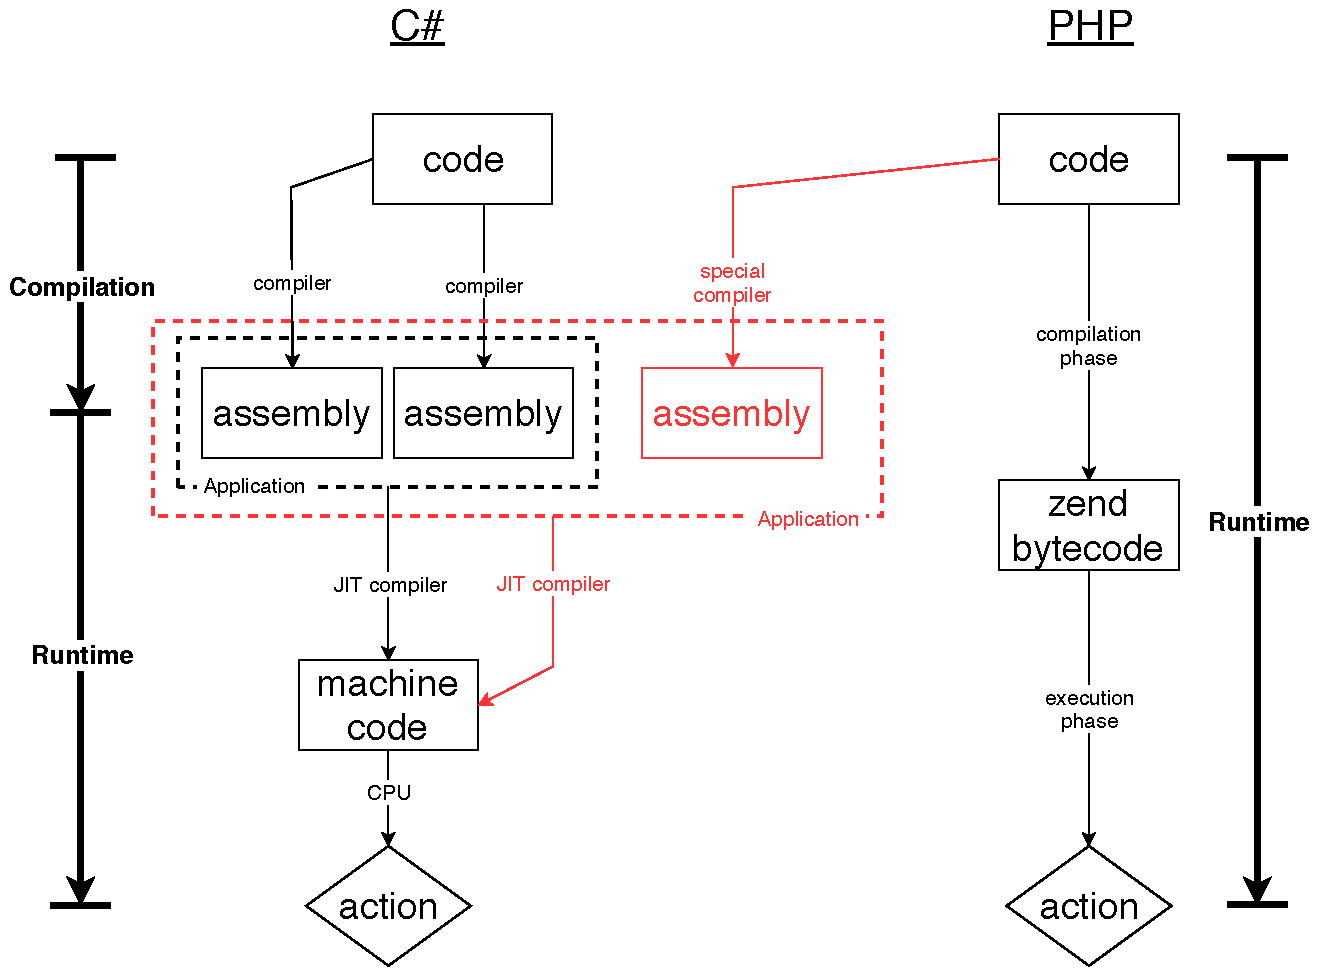
\includegraphics[width=\linewidth]{img/PHP_to_Csharp.pdf}
  \caption{PHP to C\# deployment comparison}
  \label{fig:php_csharp_comparison}
\end{figure}


\paragraph{Consequences}
The first consequence originates from the way PHP is executed. Because everything in PHP is done on runtime, parts of the code may, and sometimes do, contain by a program flow non-accessible invalid code, that would cause PHP's interpreter to throw runtime exception when executed. It is obvious that such feature cannot be brought to the world of .NET because of the compilation that validates the code in the process. For such code, there is no other way than to either remove it from the source, or exclude the whole file from the application.

The second consequence does not originate from anything mentioned but is more of an architectural nature. CLR does require whole \texttt{finally} block to be executed and for this purpose forbids statements redirecting the execution flow elsewhere \citep{microsoft.docs}. On the other hand, PHP guarantees only \texttt{finally} block entering, not its whole execution, allowing it to contain flow control statement such as \texttt{return}, which will result in overwriting the possible \texttt{try/catch} block return value \citep{php.manual}. Again, as such behaviour is inconsistent, there is no other way than to either rewrite these statements to an equivalent form without unsupported constructs, or to exclude them if the former is not possible.

Very similar differences can be observed in iterators as well. Where C\# does place further restrictions on usage of \texttt{yield} keyword in combination with \texttt{try, catch} and \texttt{finally} blocks, PHP does not \citep{microsoft.docs, php.manual}. This diversity originates again in the language-specific procession of exception handling blocks and its possible solutions are for this reason same to the preceding paragraph. 

Last but not least stands the problem of standardization. Because PHP language does not have any complete formal standard, there is no list of all defined functions, classes and possible parameters. This makes it almost impossible task to create a compiler tool which would be able to process every PHP's built in function, because that would require having cumulative knowledge of all of these. For this reason, it is beyond the capabilities of a few individuals who usually work together on such compiler and so they have to be always prepared for further compiler enhancing and additional features implementing.



\section{Peachpie}
After theoretical analysis of the languages, providing a brief outline of possible complication that might arise during compilation and presenting some of possible solutions for each of them, we can finally proceed to the actual compiler tool, Peachpie.

Peachpie is a modern PHP compiler based on Roslyn, a set of open-source compilers and code analysis APIs, also called .NET compiler platform \citep{Peachpie, microsoft.docs}. Peachpie took heavy inspiration in its predecessor Phalanger, a PHP language compiler for .NET Framework targeting the PHP language version 5 and ASP.NET 2.0 \citep{Peachpie, Phalanger}. Peachpie allows for a full compatibility with .NET, which enables the development of hybrid applications, where part of the code is written in C\# and part in PHP \citep{Peachpie}. Finally, Peachpie allows for PHP applications to be developed directly in Microsoft Visual Studio IDE \citep{Peachpie}. This way, developers can make full use of its built in features such as profiling or debugging.

\paragraph{Development}
When Phalanger was developed, its main goal was to compile legacy PHP code into .NET, at which it ultimately succeeded. However, its development slowed down through out the time and finally stopped at PHP language version 5.6 \citep{Peachpie}. 

Several years later, Microsoft introduced compiler platform called Roslyn \citep{Peachpie}. Aside from granting tools to potentially speed up both compilation and runtime phase, it also provides a way to help developers directly perform phases of compilation, such as lexical and syntactic analysis \citep{Peachpie}. Inspired by the Roslyn platform, former maintainers of Phalanger revived the concept of PHP compiler for .NET and Peachpie's development was initiated \citep{Peachpie}. 

The compiler's development continues to the present day and new development versions of software are released several times a month, each time bringing additional functionalities and missing features implementation \citep{peachpie.github}. At the time of writing, Peachpie is capable of compiling PHP versions 5.4 up to 7.4, using it within .NET Core SDK 2.1 or newer and is compatible with .NET Core 3.1 as well\citep{Peachpie, peachpie.github}.


\paragraph{Benefits of Peachpie}
Comparing and benchmarking speed of Peachpie and PHP is rather complicated task and to achieve certain reliability, it would require to perform several tightly designed tests across multiple platforms and on a wide variety of different set-ups. Although no such work has yet been done, Peachpie has been conceptually compared to Phalanger many times and each time resulted as a definite winner \citep{Peachpie}. In addition to, iolevel has published several benchmarks that provide at least provisional comparison of Peachpie and PHP \citep{Peachpie}. To come to a conclusion, Peachpie can be, in terms of speed, considered to be comparable to PHP version 7.2.

Much more promising benefits of using Peachpie are interoperability and security \citep{Peachpie}. As was mentioned before on several occasions, compiling one language into another does theoretically enable one to use features and libraries written in both of the languages and thus significantly narrow the gap between the two communities. Peachpie does put this theoretical concept into practice and presents full interoperability between PHP and .NET. In addition to, Peachpie introduces a way of eliminating potential security vulnerabilities by compiling the code into .NET \citep{Peachpie}. Between provided security improvements can be named the ability to deploy PHP applications without sources or using the security restrictions configured for the process \citep{Peachpie}.





\chapter{Problem analysis}
Regarding the name of the project, we decided to hold a convention laid down by the previous project made by the PeachPie developers, where the objective was to compile Wordpress framework into .NET. The resulting project was named Peachpied Wordpress, therefore, this project was entitled Peachpied Symfony and all custom tools provided use the Peachpied.Symfony prefix in their names.

\paragraph{Symfony project structure} As was mentioned before, each Symfony project is made from libraries, generally called Symfony Components. All these libraries reside in the \texttt{vendor} directory of the project. The rest of the project contains mainly settings such as, routing definition, environmental variables or database credentials configuration files, and user defined content, such as controller classes responsible for handling requests, images, definition of styling and front-end scripts. Aside from this, every Symfony project also contains a set of autoload files. Those are responsible for the proper load-up of all of the remaining libraries included in the vendor folder and are stored under the \texttt{vendor} directory.

\paragraph{Current problems} Ability to compile Symfony projects into .NET would yield undeniable contributions to both the communities. In terms of plain feasibility, this is what Peachpie compiler already does, nevertheless, aside from its dependence on using PHP and composer to generate certain files, there are also other problems that recede this approach from being usable in practise. These will be discussed right ahead.

When using plain Peachpie to compile Symfony project, the major problems lay in efficiency. Each time Symfony project is compiled, the whole content of the \texttt{vendor} folder is recompiled. For a bare bones project this means over a 15MB of \texttt{.php} code sources distributed over 3000+ files. This equals tenths of minutes of compilation each time. And we are talking only about the bare bones project with approximately 30 Symfony Components. The actual projects may use hundreds of them making this approach impossible in practise. We must not forget the disk space consumed by the resulting \texttt{.dll} which would be appropriate to the size of the project. Finally, due to differences in type systems and execution models of PHP and .NET, compilation errors calling either for some files' exclusion from the compilation or their direct modifications are to be expected as well.

Aside from using Peachpie in the previously mentioned manner to embed an existing Symfony project into our new .NET Core application, there is also a way of using Peachpie to include only a certain functionality from Symfony. This can be done by embedding only a set of Symfony Components in our application. This approach seems more promising as there would definitely be less files to be compiled and thus less compilation errors that needs to be tend to. Nevertheless, these files would require to be compiled over and over as well. Furthermore, there would certainly be an urge to write an API for using the desired functionality from .NET which would require a non-trivial knowledge of both Peachpie and the Symfony Component.


\paragraph{Aim of the project} When measured by the complexity of the task in terms of time needed for its completion or spatial and performance overheads, Peachpie compiler would definitely need a help of more specialized tool to deliver the solution in practically usable form. The aim of this project is to address this need and reduce both compilation time of mentioned ways of embedding Symfony within .NET Core application while increasing its actual usability by providing simple API for its usage. The spacial requirements were also considered but did play only secondary role during proposed solution's design. 



\section{Proposed Solution}
Taking its inner structure into account, one can perceive the Symfony project as two completely distinct parts. First, the \texttt{vendor} directory containing all of the libraries that the project uses, and second, basically the rest of the project folder. Moreover, for the set of Symfony components and fixed versions, the vendor folder will always look the same. Ultimately, each of these Symfony Components can be recognized as an independent unit as well, only holding references to another libraries that it requires for its proper functioning via its own \texttt{composer.json} file.

The whole solution of the previously mentioned problem is therefore based on these conclusions:

\begin{enumerate}[1:]
\item User does not manually modify content of the vendor directory.
\item The \texttt{vendor} directory for a set of Symfony Components with fixed versions will be always identical (excluding the autoloaders part). 
\item Symfony Components are self sustained with functionalities depending only on libraries listed in included \texttt{composer.json} file.
\end{enumerate}


\paragraph{Component compilation} Taking this inner composition into account, we decided that pre-compiling Symfony components and proving each one on demand would bring the most desirable outcome. This step will save considerable amount of time by deferring to the pre-compilation while bringing the highest flexibility regarding future extensibility. NuGet package manager was selected to handle this as a most widespread package manager under .NET environment. This way each composer dependency will be simulated by a package reference and NuGet will handle the rest while also saving physical space thanks to its caching system.

One drawback of introduced approach is the necessity of significant number of packages to be pre-compiled in order to comply the requirements even of the bare bones Symfony 4.2.3 project, created with the \texttt{composer create-project Symfony/Skeleton [projectName] [<version>]} command. Such project is called Symfony Skeleton and consists of 24 components. There is no feasible solution to this other than providing an at least partially automatized way of producing packages for Symfony Components.

\paragraph{Project compilation} With this approach, we will be able to supply Symfony project with pre-compiled libraries in a form of NuGet packages of required versions while saving both the compilation time and the size of resulting \texttt{.dll}. This also does resolve some of the previous dependence on PHP and composer, however, it brings several new questions that has to be addressed in order to move forward. How to handle composer's autoloading? What about Symfony's caching directory containing \texttt{.php} files produced on application start-up? And how will be composer's dependencies and the \texttt{composer.lock} file mapped to package references?

Autoloading scripts in Symfony are produced by composer's \texttt{dump-autoload} or \texttt{install} command and updated each time new Symfony Component is installed. It is true that their content is determined by a set of used components and their versions, however, we can see that providing them in a pre-compiled state as NuGet packages as well would prove very challenging. Choosing this approach would require to produce and store NuGet packages for autoloading scripts of all possible combinations of packages and their compatible versions. One, and probably the best, alternative to this approach is using composer itself to produce these scripts during an early phase of project's compilation and then simply compile them with the project. Time overhead of this method is negligible, compared to time needed for autoloading scripts pre-compiling.

Symfony projects use caching mechanism in order to speed up future request handling. These application cache are by default stored in the \texttt{var} directory and produced after first application startup. In order for the application to work correctly under .NET, these files need to be compiled as well. For Peachpie however, this means the application has to be started first either from PHP or from .NET after previous compilation, and then recompiled again with generated cache files. An easy and efficient solution to this lays once again in producing these files manually during an early phase of of project's compilation.

On he contrary of previous conclusions, solution to the final question of how to convert composer's dependencies to package references might lay already within Peachpie. One of the targets provided by the Peachpie SDK parses \texttt{composer.json} file and converts every dependency into package reference. Unfortunately, it does so only for packages not marked as development dependencies. In addition to, it does not check whether does a NuGet package for listed dependency exist in any of registered repositories. This is problematic because in .NET every package used somewhere in the code needs to be referred and thus cannot be considered a development dependency. Moreover, some packages non-development components provide only additional CLI (Command Line Interface) functionalities for composer and PHP, and therefore do not need to be referred nor compiled. Correct way to handle this issue would be to cooperate with Peachpie developers and adjust current tool to befit out needs. We decided to avoid this way in sake of saving the time such task would consume and postpone it into possible future works. Writing a custom tool handling this seems as a quick alternative, nevertheless it would require delivering it before NuGet's \texttt{restore} target is executed which means loading it directly from a \texttt{.dll}. From the perspective of UX (User Experience), this approach brings unpleasant complications, and after comparing it with complexity of setting up package references manually, we decided to settle for the manual solution for now. 


\paragraph{} Its is clear now, that regarding the number of Symfony Components and continuing development of Peachpie, delivering our tool in a production grade quality would require tremendous amount of time or a greater team of developers. Because that exceeds both our capabilities and the scope of the thesis we focused primarily on outlining how the tools should work and displaying some possibilities to provide further interoperability. The whole project is therefore to be regarded as a proof of concept.

\chapter{Component compilation}
This chapter looks closely into a phase of the problem solving that can be regarded as a preparation step. The way Symfony Components are packed into NuGet packages and the tools that help to automatize the process are discussed here. 

At first, a brief introduction into MSBuild tool will be provided as it forms a required knowledge for further understanding. After that, we will present more detailed overview of solution design. Description of various configuration files that accompany the build process will follow, ending the chapter with a section about implemented automatization of the whole Components compilation.

\paragraph{} The source code for the NuGet packages of Symfony components provided with the project can be found under the \texttt{Peachpied.Symfony/Components/4.2.3} directory. It was included in the project due to certain modifications that distinguish it from the one acquired by the \texttt{composer require "[name]:[version]"} command. More about these changes and their purpose will be discussed later on. For clarification, when speaking of a certain package folder or a \texttt{vendor} directory in the following text, those in this particular directory are meant unless stated otherwise. Moreover, custom notation \texttt{\{* ... *\}} will be used in examples on places where the thought behind the expression is of higher importance than actual implementation.


\section{MSBuild}
When a .NET project is compiled, MSBuild build system takes the configuration stored in \texttt{.[projectType]proj} file that is associated with the project and performs the compilation \citep{microsoft.docs}. The project type by convention reflects the actual extension of the file and is used in order to increase their understandability \citep{microsoft.docs}. Some of generally used extensions are \texttt{.csproj} for C\# projects, \texttt{.vbproj} for Visual Basic .NET projects, and \texttt{.msbuildproj} for projects not tied to any specific language. The \texttt{.msbuildproj} file extension is also used by Peachpie Software Development Kit (SDK). In addition, \texttt{.targets} and \texttt{.props} extensions are recognized as reusable project files that can be imported to other project files \citep{microsoft.docs}. Regardless the final extension and usage, all of the \texttt{.[projectType]proj} files are XML files that adhere to the MSBuild XML schema \citep{microsoft.docs}.

The basic syntax of MSBuild XML schema uses properties and items as a way of passing information to tasks. Where properties are name-value pairs, items are collections of values and can contain attributes. There are many additional differences between properties and items such as their typical usage, the way they are passed to tasks or the way they are processed. MSBuild reserves some property names as a mean of storing information about the project file \citep{microsoft.docs}, those are for example \texttt{MSBuildThisFileDirectory} or \texttt{MSBuildProjectDirectory}. Properties can be referenced by using the \texttt{\$([propertyName])} notation, items by \texttt{@([ItemName])}. Furthermore, new items and properties can be defined by using their name as a child element of either \texttt{PropertyGroup} for properties or \texttt{ItemGroup} for items.

Aside from that, MSBuild provides a way to modify compilation process by hooking custom targets into the build order. Target is a set of tasks, functional units providing certain actions, represented by a \texttt{Target} element. On the .NET project compilation, a list of default targets is sequentially executed performing each target's actions or skipping them based on provided conditions, resulting in the project's compilation. MSBuild has a built-in collection of tasks providing basic actions such as \texttt{Delete}, \texttt{Copy} or \texttt{Message}. In addition to, custom tasks can be registered from assemblies via the \texttt{UsingTask} element. We can include custom tasks written as .NET class libraries that will provide us with the required missing functionalities. Such class only needs to either implement the \texttt{Microsoft.Build.Framework.ITask} interface or inherit from the \texttt{Microsoft.Build.Framework.Task} class and define an \texttt{Execute} method returning a \texttt{boolean} value. Task's input parameters are supplied through attributes and correspond to the .NET properties in the class definition. Output parameters of the task are created by marking selected .NET properties with the \texttt{[Output]} attribute. These can be collected after task's execution with the \texttt{Output} subelements which perform mapping from .NET property to either MSBuild item or property.


\section{Solution design}
For each library, we need to create a project, more precisely, we need a \texttt{.msbuildproj} file that will be supplied to the MSBuild task. Initially, to include Peachpie compiler we need to set the \texttt{Sdk} attribute of the root \texttt{Project} element to \texttt{Peachpie.NET.Sdk/[version]}. This way, the properties and the targets used by Peachpie compiler will be imported into the project. The second step is to set the \texttt{GeneratePackageOnBuild} property to true in order for MSBuild to output a NuGet package. Then we need to specify files that are to be compiled, excluded and copied to the output package in a form of static content. For this purpose, items \texttt{Compile} and \texttt{Content}, and their attributes \texttt{Include}, \texttt{Exclude} and \texttt{Remove} can be used. When MSBuild copies static files to the output, it by default preserves the structure the files are located in. As the NuGet packages will be used and referenced from the user defined content of the project, it is preferable to place all the \texttt{.msbuildproj} files for each project to parent directory of \texttt{vendor}. This way the path to static files will remain unchanged, that is, beginning with \texttt{vendor}. The last step is to specify package's dependencies. This can be done with either \texttt{ProjectReference} for dependencies on another projects, or with \texttt{PackageReference} for dependencies on NuGet packages \citep{microsoft.docs}.

On the first look, this seems like a great amount of repetitive code. For the sake of the DRY principle, we will make use of \texttt{.props} and \texttt{.target} files and try to generalise as much of the configuration as possible. Either can be used, as MSBuild does not really pay much attention to the actual extension of a file, but to follow the conventional usage, we will store reusable properties in \texttt{.props} files and define reusable targets in a \texttt{.targets} file.


\section{Props files} As was mentioned before, we have to set the \texttt{GeneratePackageOnBuild} property for every project in order to generate NuGet packages. Aside from this, there are several other significant and required properties that we need to set-up as well to produce the correct output. These properties specify the output type of the project, target framework, project description, name of both the output \texttt{.dll} and the final package, version of the package and necessary routes where to output NuGet package. We also have to set up a path for intermediate output and the path to the output directory. All of these properties will be fairly similar for all of the packages, varying only in the names and parts of paths.

In order to fully isolate previously mentioned properties into a separate file, we denoted a naming convention for the \texttt{.msbuildproj} files. This way, we was able to use the project name to derive name of the output package and a path to the actual library folder. For that, we used MSBuild's reserved property \texttt{MSBuildProjectName} that holds the file name of the project without the extension.

Now, we can proceed to configuring the two properties that will differ among the projects, libraries' names and their sources locations. Hence, we will create two properties \texttt{LibraryName} and \texttt{LibraryPath}. The naming convention for the Symfony components follows the rule \texttt{[providerName]\string\[componentName]}. For this reason, and also to comply the NuGet package naming rules, we will define a property that will simply replace each backslash delimiter on the route from vendor folder to the library folder with dots. Extended with properties holding fixed value like \texttt{OutputType} or \texttt{TargetFramework} we have so far a fully automatable process. To detach background properties from ones used for project configuration and compilation items configuration from all of them we created 3 \texttt{.props} configuration files.


\paragraph{Directory.Build.props} This file is optional and should be located at the root folder of the project. Its content is imported automatically in an early stage of compilation, making it capable of overwriting properties defined in most of the build logic \citep{microsoft.docs}. The backslash to dot conversion logic will be defined there, introducing \texttt{ProjectNameLocation} property as a result. Additionally, values for the \texttt{BaseIntermediateOutputPath} and \texttt{BaseOutputPath} needs to be set there as well as they are later used for calculating routes used for storing NuGet related data \citep{microsoft.docs}. Because we compile all the Symfony components from the same working directory, we have to separate their output paths in order to avoid file overwriting. This is where we use the \texttt{ProjectNameLocation} for the first time and its also the reason this property must be defined here. The actual code that handles following can be seen in the subsequent Listing.

\begin{center}
\lstset{language=XML,
	morekeywords={encoding, xmlns, version}}
\begin{lstlisting}[caption={Directory.Build.props},captionpos=b]
<Project xmlns="http://schemas.microsoft.com/developer/msbuild/2003">

	<PropertyGroup>
		<ProjectNameLocation>
			$([MSBuild]::EnsureTrailingSlash('\$([System.String]::Copy('\$(MSBuildProjectName)').Replace('.','\'))'))
		</ProjectNameLocation>
		<BaseOutputPath>
			.\bin\$(Configuration)\$(ProjectNameLocation)
		</BaseOutputPath>
		<BaseIntermediateOutputPath>
			.\obj\$(Configuration)\$(ProjectNameLocation)
		</BaseIntermediateOutputPath>
	</PropertyGroup>

</Project>
\end{lstlisting}
\end{center}


\paragraph{propertiesConfig.props} Before proceeding to the build properties file, we need to mention that PeachPie compiler provides by default a feature of \texttt{composer.json} file parsing and producing package references as an output. Because this feature would collide with our own package references retrieval mechanism we need to provide PeachPie compiler with an invalid route to \texttt{composer.json}. This is done by setting the \texttt{ComposerJsonPath} property to any invalid value, for readability purposes we set this property to \texttt{Ignore}. Now, with the use of defined \texttt{ProjectNameLocation} property, the build properties \texttt{.props} file will be organized as follows.

\begin{center}
\lstset{
	language=XML,
	morekeywords={encoding, version, xmlns}}
\begin{lstlisting}[caption={propertiesConfig.props},captionpos=b]
<Project xmlns="http://schemas.microsoft.com/developer/msbuild/2003">

	<PropertyGroup>
		<OutputType>Library</OutputType>
		<TargetFramework>netstandard2.0</TargetFramework>
		<Description>.NET class library in PHP</Description>
		<LibraryName>$(MSBuildProjectName)</LibraryName>
		<LibraryPath>
			vendor\$(ProjectNameLocation.toLower())
		</LibraryPath>
		<AssemblyName>$(LibraryName)</AssemblyName>
		<PackageId>$(LibraryName)</PackageId>
		<GeneratePackageOnBuild>True</GeneratePackageOnBuild>
		<PackageOutputPath>
			..\..\..\Nuget-Repository\Components\
		</PackageOutputPath>
		<IntermediateOutputPath>
			.\obj\$(Configuration)\$(ProjectNameLocation)
		</IntermediateOutputPath>
		<OutputPath>
			.\bin\$(Configuration)\$(ProjectNameLocation)
		</OutputPath>
		<OutDir>$(OutputPath)</OutDir>
		<ComposerJsonPath>Ignore</ComposerJsonPath>
	</PropertyGroup>

</Project>
\end{lstlisting}
\end{center}


\paragraph{compilationConfig.props} Now, that we have successfully set up all the directories and names used on compilation, we can move on to the definition of what to be compiled and included in the package. We can expect that all of the projects will share the same patterns in compile and content files specification, that is in general, they will compile all of the \texttt{.php} files located in the library folder and include all the files as content. However, such assumptions proved to be much more naive that it might seem.

We must not forget that we are compiling one language into another which in this case brought a problem of using features of one language, in our case PHP, that simply cannot be brought into the world of .NET. The most frequently encountered error associated with this was an inclusion of a non-existing class or interface. In PHP's testing classes it is very common to include external libraries that are not mentioned in the \texttt{composer.json} file as dependencies. This is because test classes are not executed in typical program flow and require explicit actions for their execution. It does not change the fact that triggering such action manually will cause the original PHP project to crash. In some cases however, PHP does check presence of a class prior to its actual usage, protecting itself from executing a file that includes such class. Unfortunately, this is not supported in .NET as each file compiles independently and the fact that it is not executed does not change the fact that it must be compiled.

There are two possible solutions for this problem. Either we can look up the dependency tree of each such test class, compile them into separate NuGet packages and reference them, or we can exclude the tests. The later solutions proves to be better for most of users as a typical user does not perform downloaded libraries' testing. Therefore, their inclusion would cause unnecessary overhead in the the number of NuGet packages required for the project's compilation and also in the time of the actual project compilation. The test files are the only files we can generally exclude from every project, but in most cases, are also the only files required to be excluded in order to achieve a successful compilation. After we extended the naive configuration from the previous paragraph with the test exclusion we ended up with a specification shown in the Listing 5.3.
 
\begin{center}
\lstset{
	language=XML,
	morekeywords={encoding, version, xmlns, Include, Exclude,
	CopyToOutputDirectory}}
\begin{lstlisting}[caption={compilationConfig.props},captionpos=b]
<Project xmlns="http://schemas.microsoft.com/developer/msbuild/2003">

	<ItemGroup>
		<Compile Include="$(LibraryPath)**\*.php"
			Exclude="   $(LibraryPath)**\test\**;
				        $(LibraryPath)**\Test\**;
				        $(LibraryPath)**\tests\**;
				        $(LibraryPath)**\Tests\**;"/>
		<Content Include="$(LibraryPath)**"
			Exclude="   **\*.msbuildproj;
				        **\*.csbuildproj;
				        **\*.props;
				        $(LibraryPath)obj\**;
				        $(LibraryPath)bin\**;" 
			CopyToOutputDirectory="PreserveNewest">
			
			<BuildAction>Content</BuildAction>
			<PackagePath>
				contentFiles\any\netcoreapp2.0\$(LibraryPath)
			</PackagePath>
			<PackageCopyToOutput>true</PackageCopyToOutput>
			<Visible>true</Visible>
			<Pack>true</Pack>
			<Link>
				$(LibraryPath)%(RecursiveDir)%(Filename)%(Extension)
			</Link>
		</Content>
	</ItemGroup>
 
</Project>
\end{lstlisting}
\end{center}

\paragraph{Required code edits} Unfortunately, not all the compilation errors could be resolved by excluding the problematic source code. Sometimes, core parts of Symfony components use language constructs that PHP supports and .NET does not. For these files the only remaining solution is to edit the code itself and refactor the functionally to similar but compilable version.

Several times, Symfony components used \texttt{yield} keyword inside a \texttt{try-catch} block. Such operation cannot be performed under the .NET environment as it places strict restrictions on usage of iterators inside those blocks. These cases have been rewritten into equivalent form with the use of arrays and booleans as flags. Furthermore, as such edits can be automatized, PeachPie developers have later implemented workarounds to handle this code without compilation errors.

The second encountered compilation errors were caused by inappropriate usage of the \texttt{\_\_toString()} function. There are special rules applying to this function and its return values in PHP which Peachpie compiler strictly complies with. Symfony on the other hand, occasionally throws an exception there which when compiled resulted in an invalid return type error. Such code was, for the sake of further progress, temporarily rewritten to simple empty string returning and later resolved in another PeachPie compiler update.

Next problem encountered was of the same nature as the first one mentioned, that is, in the disruption of the program flow. Symfony's Flex component used \texttt{return} statement from the \texttt{finally} block of exception handling construct. However, this component is used solely as a supplement for the Composer tool, and thus, for the purpose of managing additional libraries. Compiled Symfony project has therefore no use for such functionality as requiring additional packages from compiled project via Composer or Flex is redundant with the introduction of NuGet packages. Thanks to that, the Flex component can be completely omitted from the compilation.

The last type of compilation errors was caused by a missing implementation of a small set of features within Peachpie compiler. Each of them was later fixed in a newer release of the software. This could not be helped as the Peachpie compiler is still in the phase of development and such problems were expected to appear. Along some of these missing features we can name missing implementations of the \texttt{SessionUpdateTimestampHandlerInterface} interface or \texttt{PCRE\_ANCHORED(A)} flag in Peachpie's perlregex. 


\section{Targets file and ComponentTools}
Even with the mentioned code edits and 3 \texttt{.props} files ready, we cannot proceed to actual Symfony component compilation yet. There have been several details that were intentionally left out or skipped in the previous sections and addressing them is a job of the \texttt{automatizationConfig.targets} file and the \texttt{Peachpied.Symfony.ComponentTools} project. The skipped details were packages' versions and packages' dependencies, and omitted was explanation what to do with those Symfony components that require more precise compilation configuration than just excluding all test sources.

\paragraph{automatizationConfig.targets} This configuration file specifies custom targets and hooks them into each component's compilation process. This can be achieved in multiple different ways but the most common is either by the \texttt{BeforeTargets} or \texttt{AfterTargets} attribute of the \texttt{Target} element. Aside from basic \texttt{BeforeTargets} and \texttt{AfterTargets}, MSBuild specifies additional means of target execution flow modifications. One of them is \texttt{DependsOnTargets} attribute, resulting in sequential triggering of all the mentioned targets prior to the target's body execution. Each target can also define \texttt{Inputs} and \texttt{Outputs} attributes. When present, the timestamps of the specified input and output files are compared, possibly resulting in marking the target as up to date and thus skipping its execution. Finally, \texttt{Condition} attribute can be used to control target's execution with a \texttt{boolean} expression (this attribute can also be used on tasks' elements, itemGroups and many other elements).

Now we can proceed to the actual \texttt{automatizationConfig.targets} file content. Each of the 3 missing details mentioned is provided by different task but all of them are located in the \texttt{Peachpied.Symfony.ComponentTools.dll}. The actual implementation of these tasks will be discussed in the upcoming section. Naturally, the task responsible for retrieving component's package references needs to be executed before the \texttt{Restore} target and all of its preprocessing during the component's compilation. Unfortunately, this makes it impossible to distribute the \texttt{.dll} as a NuGet package. The ideal solution for this problem would be to include the \texttt{.dll} inside of the Peachpie SDK but due to a large extent of such operation we decided to distribute it only in a way of source code and static \texttt{.dll} in this repository.

Each one of the custom tasks is dependant on existence of the \texttt{libsCache.json} file produced by the \texttt{TWarmLibsCache} target. This \texttt{.json} file contains necessary information that is further transformed by other 3 tasks into required properties and items. Caching target's execution is bound by the \texttt{composer.lock} and \texttt{libcCache.json} files' timestamps using technique mentioned before, ensuring cache file is regenerated only when necessary. Sadly, it is not possible to use a collection of Symfony components' \texttt{composer.json} files instead of \texttt{composer.lock} because the \texttt{.lock} file contains the \texttt{version} key supplied by the Composer during package installation which is absent from components' \texttt{.json} files.

Finally, parts of the \texttt{automatizationConfig.targets} file providing discussed functionality can be seen in the following Listing.

\begin{center}
\lstset{
	language=XML,
	morekeywords={TaskName, AssemblyFile, Name, Compile, CachePath, 
	Inputs, Outputs, Files, Condition, BeforeTargets, LibName, LibPath,
	ProjPath, ConfigPath, AfterTargets, DependsOnTargets, Remove,
	ItemName, TaskParameter, LibVersion, Include, RepoPath, 
	PropertyName}}
\begin{lstlisting}[caption={automatizationConfig.targets},captionpos=b]
...
<UsingTask TaskName="WarmLibsCache" AssemblyFile="$(LibsAssebly)" />
<UsingTask TaskName="GetLibVersion" AssemblyFile="$(LibsAssebly)" />
<UsingTask TaskName="GetLibReferences" AssemblyFile="$(LibsAssebly)" />
<UsingTask TaskName="FilterLibExcludes" AssemblyFile="$(LibsAssebly)" />
	
<Target Name="TWarmLibsCache" Outputs="$(CacheDir)\libsCache.json"
		Inputs="$(MSBuildProjectDirectory)\composer.lock">
	<Delete Files="$(CacheDir)\libsCache.json" 
			Condition="Exists('$(CacheDir)\libsCache.json')" />
	<WarmLibsCache ProjPath="$(ProjPath)" ConfigPath="$(ConfigPath)"
			CachePath="$(CacheDir)" />
</Target>
...
<Target Name="TGetLibReferences" BeforeTargets="CollectPackageReferences"
		DependsOnTargets="TWarmLibsCache">
	<GetLibReferences CachePath="$(CacheDir)" RepoPath="$(RepoPath)" 
			LibName="$(MSBuildProjectName)" 
			Condition="$(ManualReferences)!=true">
		<Output TaskParameter="References" ItemName="PackageReference" />
	</GetLibReferences>
</Target>
	
<Target Name="TSymfonyAutomatization" BeforeTargets="BeforeBuild" 	 	 
		DependsOnTargets="TWarmLibsCache">
	<GetLibVersion CachePath="$(CacheDir)" 
			LibName="$(MSBuildProjectName)" 
			Condition="$(ManualVersion)!=true">
		<Output TaskParameter="Version" PropertyName="PackageVersion" />
	</GetLibVersion>

	<FilterLibExcludes ConfigPath="$(ConfigPath)" 
			LibPath="$(LibraryPath)" LibVersion="$(PackageVersion)" 
			LibName="$(MSBuildProjectName)" 
			Compile="@(Compile)" Condition="$(ManualExcludes)!=true">
		<Output TaskParameter="NewCompile" ItemName="NewCompile" />
	</FilterLibExcludes>
	<ItemGroup>
		<Compile Remove="@(Compile)" />
		<Compile Include="@(NewCompile)" />
	</ItemGroup>
</Target>
\end{lstlisting}
\end{center}

\paragraph{ComponentTools} The first task provided by the project's \texttt{.dll} is \texttt{WarmLibsCache}. As its title and input parameters from the previous Listing suggest, this task loads the \texttt{libsConfig.json} configuration file from \texttt{ConfigPath} and the \texttt{composer.lock} file from \texttt{ProjPath}, and creates a cache file at \texttt{CachePath}. This cache file lists all the installed Symfony Components, sorted in a cumulative manner, according to their dependencies. For each component, there is an object indexed by its name, holding the component's version, indicator whether it was listed as a development dependency in the \texttt{composer.lock} file and a list of names of packages it depends on. Where the first two values are simply parsed out from the \texttt{composer.lock} file, the process of gathering each component's references proved to be much more complicated and will be described in detail right ahead.

What might seem as a task that could be solved simply by loading an array of names from the \texttt{require} key in he component's record of the \texttt{composer.lock} file turned out much more complicated after realising that for a successful compilation components do also require references to the packages listed under the \texttt{require-dev} key. This does not come as a surprise because from the .NET's point of view it does not really matter whether some functionality is actually used or not during the compilation. However, joining these two arrays of package names would have not present a challenge, were it not for the circular dependency errors that appeared during compilation. Because of that, the whole process of package dependency tree building and optimizing had to be implemented.

In the first phase of the algorithm a simple dependency tree is build. This is done using custom data structure for each node, holding its name, version and a list of children nodes, its dependencies. After the tree is incrementally built, each node is traversed recursively creating a list of unique cycles. At last, all edges in each cycle marked as development dependencies are selected and the one leading to the package with the longest name is removed. This "random" approach proved to be working for every circular dependency error containing at least one development edge encountered.

Some of the errors unfortunately did not contain any development edge and thus required additional information on how to handle such cycles. This is provided via the \texttt{libsConfig.json} configuration file mentioned before.

Finally, a list of objects with versions, development indicators and valid dependencies is sorted in order to allow sequential build and saved to the \texttt{libsCache.json} file. This class grants access to this list via a public property along with a list of packages and development packages  loaded from the \texttt{composer.lock} file. We will skip the reasons for this and return to it at the end of the chapter.

As we allready know, the \texttt{libsConfig.json} file contains additional configuration for the Symfony components' compilation defined by user. At the same time, it is also the only actual information that has to be provided manually. Aside from the mentioned hints for circular dependencies resolving, additional excludes or overriding includes of default excludes can be specified there. This can be done either separately for each version of each component or globally for every version without its explicit configuration. 

Thanks to this manual configuration and the cache file, the \texttt{GetLibVersion} and \texttt{GetLibReference} tasks consist basically of looking up a component's record in the cache file and then storing an appropriate value either in the \texttt{PackageVersion} property or the \texttt{PackageReference} item. The remaining \texttt{FilterLibExcludes} task is specific in its functionality because it does not provide any new configuration property or item. Rather, it modifies the value of the \texttt{Compile} item by applying additional excludes and includes from the \texttt{libsConfig.json} file. After that, content of the former \texttt{Compile} item is replaced with a new content in order to prevent duplicate file entries, which would result in compilation errors.


\section{Automatization of the process}
Thanks to all the tools and external configuration mentioned, our project file that will compile a single Symfony component into a NuGet package reduces to a few lines displayed in the next Listing.

\begin{center}
\lstset{
	language=XML,
	morekeywords={encoding, version, Sdk, Project,
	CopyToOutputDirectory}}
\begin{lstlisting}[caption={compilationConfig.props},captionpos=b]
<Project Sdk="Peachpie.NET.Sdk/">      
    <Import Project="....\Props\automatizationConfig.targets" />
    <Import Project="....\Props\propertiesConfig.props" />   
    <Import Project="....\Props\compilationConfig.props" />
</Project>
\end{lstlisting}
\end{center}

Such files could be produced automatically for every Symfony component in a given directory or project. The tool providing this functionality was named \texttt{Peachpied.Symfony.BuildGen} and its process of execution is displayed in the Figure 5.1, which will be further explained in the rest of this chapter.

\begin{figure}[!ht]
  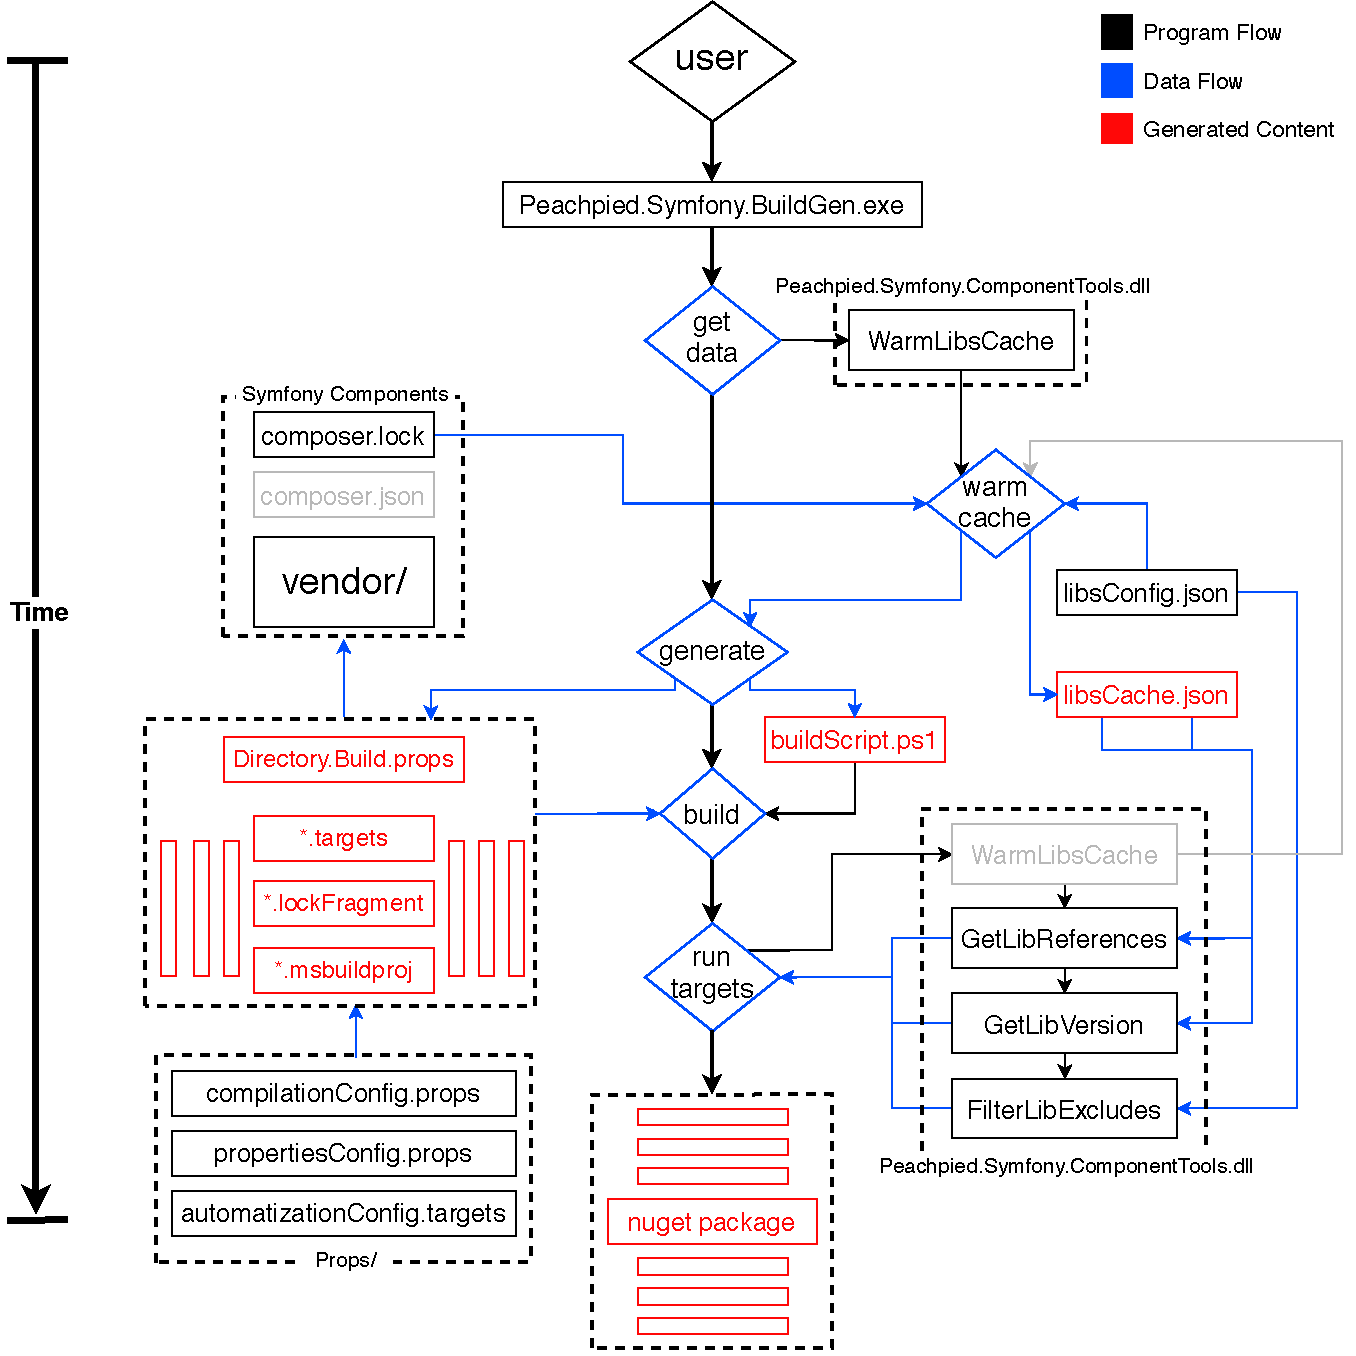
\includegraphics[width=\linewidth]{img/Components-compilation.pdf}
  \caption{Compilation process of Symfony components}
  \label{fig:Components-compilation}
\end{figure}


\paragraph{Peachpied.Symfony.BuildGen} This utility is distributed as an executable file that generates \texttt{.msbuildproj} and other necessary  files for every Symfony component found in the target directory. These are marked red in the Figure 5.1. In addition to, the utility also outputs the \texttt{buildScript.ps1} script that can be run in order to execute \texttt{dotnet build} on each produced \texttt{msbuildproj} in correct order. The target directory for the build generator is supplied by the \texttt{-p, --project} parameter. Aside from that, the utility also accepts optional paths to the \texttt{libsConfig.json} and \texttt{.props} files that are otherwise set to default values regarding the repository structure. Flag parameter \texttt{-b, --build} automatically runs generated \texttt{buildScript.ps1} on created files, and with the \texttt{-d, --debug} flag it is possible to skip final clean-up phase that automatically removes all generated files when the \texttt{-b} parameter is included.

List of Symfony Components present in the target directory is obtained using the \texttt{WarmLibsCache} class. This step is marked \texttt{\frenchspacing1.} and \texttt{\frenchspacing2.} in the Figure. In the step \texttt{\frenchspacing3.} of the Figure, we prepared public properties of the class with the help of \texttt{composer.lock} and \texttt{libsConfig.json} files. Load-up of these files is marked with the blue arrows leading towards the \texttt{warm cache} action in the Figure. As a side effect of the \texttt{WarmLibsCache} class execution, the \texttt{libsCache.json} file is produced for the obtained list of Symfony Components.

Step \texttt{\frenchspacing4.} of the Figure marks transfer to the generating phase of the compilation. Regarding the actual files provided by the build generator utility, it firstly creates the \texttt{Directory.Build.Props} file. After that, the necessary information like the list of package data and the ordered collection of package names are loaded from the \texttt{WarmLibsCache} class and one \texttt{[PackageName].msbuildproj}, one \texttt{[PackageName].lockFragment.json} or \texttt{[PackageName].lockFragment-dev.json}, and one \texttt{[PackageName].targets} file is generated for each Symfony Component. All generated files are placed in the target directory provided in order to comply previously mentioned requirement for paths to NuGet packages' static files.

The \texttt{.lockFragment} files hold each component's record parsed out from the \texttt{composer.lock} file. The \texttt{.targets} files are special as every NuGet package can include one such \texttt{.props} and \texttt{.targets} file that will be automatically imported into the project referring the NuGet. The requirements for this to work are to name the files accordingly to the package names and place them inside the \texttt{build} directory of the package. The files can be also copied to the \texttt{buildTransitive} directory which will result in transitive behaviour of the functionality. However, this feature is only available in NuGet version 5.0 and newer. Each \texttt{.targets} file provides a functionality to restore Symfony Component's folder inside the \texttt{vendor} directory of the project that uses the NuGet. In addition to, it also exposes the \texttt{LockFragments} item with appended path to its \texttt{.lockFragment.json} file. These functionalities are required for additional automation during actual Symfony project compilation and thus will be discussed in greater detail in the next chapter. A truncated example of one such \texttt{.targets} file can be found in the following Listing.

\begin{center}
\lstset{
	language=XML,
	morekeywords={encoding, version, xmlns, InitialTargets,
	Include, Condition, Name, Text, Importance, SourceFiles,
	DestinationFolder}}
\begin{lstlisting}[caption={Psr.Cache.targets},captionpos=b]
<?xml version="1.0" encoding="utf-8"?>
<Project xmlns="http://schemas.microsoft.com/developer/msbuild/2003" 
		InitialTargets="Copy_Psr_Cache_Vendor">
    
    <ItemGroup>
        <LockFragments Condition="{* file exists *}"
        		Include="{* package/build/ *}
        		../tools/any/any/Psr.Cache.lockFragment.json" />
        <LockFragments Condition="{* file exists *}"
        		Include="{* package/build/ *}
        		../tools/any/any/Psr.Cache.lockFragment-dev.json" />
    </ItemGroup>

    <Target Name="Copy_Psr_Cache_Vendor" 
    		Condition="$(RestoreVendor)==true 
 			AND {* project/vendor/psr/cache does not exist *}">
        <Message Text="Copying Psr.Cache assets..." Importance="high" />
        <ItemGroup>
            <Copy_Psr_Cache_Vendor_Files Include="{* package/build/ *}
            ../contentFiles/any/netcoreapp2.0/vendor/**/*.*" />
        </ItemGroup>
        <Copy SourceFiles="@(Copy_Psr_Cache_Vendor_Files)" 
        		DestinationFolder="{* project/vendor *}"/>
    </Target>

</Project>
\end{lstlisting}
\end{center}

Furthermore, with the use of previously mentioned ordered collection of package names, the \texttt{buildScript.ps1} file is generated providing means of automatic compilation of Symfony Components in the order denoted by the dependency tree. 

In case the \texttt{-b} flag was used, the utility next runs the \texttt{buildScript.ps1} script and proceeds to the compilation, marked with number \texttt{\frenchspacing5.} in the Figure. This is performed as described in the previous sections. First, the \texttt{.msbuidproj} file is loaded. After that, MSBuild targets run in execution order and handle importing of \texttt{.props} with \texttt{automatizationConfig.targets} and ultimately locating package specific \texttt{lockFragments} and \texttt{.targets} as well. Figure 5.1 depicts this phase separated from automatization targets execution in sake of increased readability. During the MSBuild targets execution named the \texttt{run targets} action in the Figure 5.1, custom targets are executed chronologically in displayed order providing missing information for the compilation and optionally skipping the \texttt{WarmLibsCache} target in case the \texttt{libsCache.json} file is already present in the target directory. This corresponds to the steps \texttt{\frenchspacing6.} to \texttt{\frenchspacing10.} in the Figure and on completion, passes control back to the MSBuild targets that finally produce NuGet packages.

We can now sum-up the actual compilation process of a set of Symfony components from the earliest phase of PHP sources downloading to producing actual NuGet packages into the following steps.

\begin{enumerate}[i:]
\item Clone the repository and initialize a directory under the \texttt{Peachpied.Symfony/Components} path with the \texttt{composer init} command (optionally skip the interactive \texttt{composer.json} configuration).
\item Require a set of Symfony components either by running \texttt{composer require [packageName:version]} or in the interactive configuration during the previous step.
\item Compile the \texttt{Peachpied.Symfony.BuildGen} sources with the \texttt{dotnet publish -r {Runtime}} command into executable file.
\item Run the build generator tool supplying the path to the target directory.
\item Modify sources uncompilable by the compiler and extend the \texttt{libsConfig.json} file with an additional configuration for problematic packages if needed.
\item Find the produced NuGet packages under the \texttt{Nuget-Repository/Components} path.
\end{enumerate}

Finally, one can notice that to compile Symfony components of an existing Symfony project first two steps will not probably need to be executed. The third step is also a one time job, and the fifth step should not be needed when Peachpie compiler is ready for the production and when the \texttt{libsConfig.json} contains all the necessary configurations after supplied by the community. Therefore, the whole compilation would in such case reduce to a single step of manual execution of the build generator tool. This can be observed on the Figure 5.1 where the execution of the tool is followed by automatic actions all the way to the NuGet packages producing.

\chapter{Project compilation}
This chapter focuses on the way actual Symfony projects are compiled and deployed using Peachpied Symfony toolkit. It introduces tools that make it possible and describes the process of their development. At the end of the chapter, an overview of provided feature of template engines interoperability is revealed.

\section{Compilation setup}
Whether we want to embed our existing Symfony application within another
 .NET Core one or just compile it for enhanced security, we always have to produce it in a form of \texttt{.dll} and supply it to the .Net Core web server. In this case, we decided to choose Kestrel web server as it is both open-source and Peachpie already contains an extension that allows Kestrel to handle requests targeting \texttt{.php} files and process them with \texttt{dll} library compiled from PHP code \citep{Peachpie}. This binding is in our case done by creating two .NET projects, one for the Symfony sources and the other for the server.

\paragraph{Binding with the web server} For that, we can use an already made template called ``Web App" provided by Peachpie. Upon usage, the template produces the \texttt{Website} and the \texttt{Server} directories. The \texttt{Server} one contains simple project with a base configuration for Kestrel server and logic for \texttt{.php} request handling. The other one is expected to contain PHP code for compilation.

Apart from the configuration files \texttt{appsettings.json} and \texttt{launchSettings.json}, and project file .csproj, the server project directory by default contains only \texttt{Program.cs} file representing an entry point of the application. It consists of two classes, the \texttt{Program} class with the \texttt{static void Main(string[] args)} function and the \texttt{Startup} class with the already discussed \texttt{ConfigureServices} and \texttt{Configure} functions. Furthermore, Listings 2.1, 2.2 and 2.3 combined represent the whole default \texttt{Program.cs}. The only difference is that the \texttt{Main} method must in the Host object configuration declare the actual Symfony project name.

\paragraph{Configuring Symfony's .msbuildproj} For the majority of pure PHP web applications, the system described will already be executable, however, few further adjustments in Website's \texttt{.msbuildproj} file have to be done in order to run our application as expected.

First, we have to modify value of the \texttt{Compile} item. Website project compiles every \texttt{.php} file by default which is clearly more than we actually need. As we supply Symfony Components via package references, we can safely exclude content of the \texttt{vendor} directory which might in case of compiling an existing Symfony project occur to exist in the \texttt{Website} directory. We must not forget about the autoloading scripts that are part of the \texttt{vendor} directory as well so we have to make an exception for them in the exclusion rule.

Secondly, we need to include all the static content of the project like configuration \texttt{.yaml} files, but images and other assets as well. This is done by setting up a \texttt{Content} item.

Thirdly, package references to the Symfony Components used by the original project need to be manually set up. This is done by copying them from the project's \texttt{composer.json} file and rewriting them to the NuGet references. For this reason the \texttt{Peachpied.Symfony.Skeleton} NuGet package was created that groups together dependencies of Symfony Skeleton project with a matching version. As this thesis focuses solely on Symfony 4.2.3, this package is prepared only in this particular version. However, automatic version resolving target was implemented as a part of provided Skeleton's \texttt{.msbuildproj} file allowing their future arrangement into folders by version names.

Finally, one must not forget about the autoloading scripts and cache directory discussed in chapter 4. For now, we will settle for knowing, that all these problems will be resolved automatically by adding package reference to the \texttt{Peachpied.Symfony.ProjectTools} NuGet package. Implementation details of this set of tools will be discussed in the following section. Bare bones Symfony application's configuration for compilation will in the end look as shown in the following Listing.

\begin{center}
\lstset{language=XML,
	morekeywords={Include, Exclude, Version, CopyToOutputDirectory}}
\begin{lstlisting}[caption={Empty-Page.msbuildproj},captionpos=b]
<PropertyGroup>
	<OutputType>Library</OutputType>
	<TargetFramework>netstandard2.0</TargetFramework>
    <AssemblyName>Empty-Page</AssemblyName>
</PropertyGroup>

<ItemGroup>
	<Compile Include="**\*.php" 
			 Exclude="vendor\**; config\bootstrap.php; 
					  .\obj\**; .\bin\**" />
	<Compile Include="vendor\composer\**\*.php; vendor\autoload.php" />
    <Content Include=".\**" 
			 Exclude="{* all non configuration files *}" 
			 CopyToOutputDirectory="PreserveNewest" />
</ItemGroup>

<ItemGroup>
    <PackageReference Include="PeachPied.Symfony.Skeleton" 
    		 Version="4.2.3" />
    <PackageReference Include="Peachpied.Symfony.ProjectTools" 
			 Version="1.0.0" />
</ItemGroup>
\end{lstlisting}
\end{center}

In order to bring UX even further, all the previously mentioned steps were compressed into two new templates provided in the \texttt{Peachpied.Symfony.Templates} NuGet package. The ``Symfony Skeleton" or ``syskeleton" template creates a doublet of base Kestrel server configuration and bare bones Symfony version 4.2.3 application with all the \texttt{.php} sources provided. The second template called ``Symfony-Empty-Project" or ``syemptyproj" creates one project with the same Kestrel configuration as the previous template, but the Symfony project produced contains only the \texttt{.msbuildproj} file without any Symfony Component package references, letting user import own sources and setup required package references as required.


\section{ProjectTools package}
Just like the mentioned \texttt{ComponentTools} hooked the custom targets in order to provide necessary configuration settings during the Symfony Components compilation, \texttt{ProjectTools} does the same thing during the Symfony project compilation in order to provide the compilation with additional \texttt{.php} files needed for actual application execution. Custom targets provided by this project are named \texttt{RestoreComposerLock}, \texttt{GenerateSymfonyAutoload} and \texttt{GenerateSymfonyCache}. Because these tasks do not manipulate with project's package references, whole project can be safely delivered in a form of NuGet package. Furthermore, we can make use of discussed NuGet's feature to import special \texttt{.targets} file into out project file. This way, we prepare all the custom targets' load-up and usage in \texttt{Peachpied.Symfony.ProjectTools.targets} and let the package manager handle their embedding into compiled project's execution order, while effectively isolating user from all the background tasks.

\paragraph{RestoreComposerLock} This task is responsible for collecting all the \texttt{lockFragments} from NuGet packages of Symfony Components and joining them together into \texttt{composer.lock} file. The data from packages are in fact extended by the data taken from project's \texttt{composer.json} file in order to provide a file that matches the one originally produced by Composer. This also required to rewrite implementation of content hashing function used in composer into C\# in order to provide value for the \texttt{content-hash} key.

This task's execution is bound by appropriate \texttt{Inputs} and \texttt{Outputs}, ensuring that it runs only when there is no \texttt{composer.lock} file present or its content is outdated compared to \texttt{composer.json}.

\paragraph{GenerateSymfonyAutoload} Things get slightly more complicated with this task due to requirements to use composer itself to produce these file for us. The implementation we settled for includes the whole \texttt{composer.phar} file as a static asset of the NuGet package and calls it on task's execution with the \texttt{php composer.phar dump-autoload} command.

Unfortunately, quite severe problem emerged regarding composer's \texttt{dump-autoload} requirements. For its proper execution, this task needs the \texttt{installed.json} file to be located under the \texttt{vendor/composer} path in the project directory. Thankfully, this file is nothing more than a concatenation of each package's \texttt{lockFragment} and thus can be easily created using previously generated \texttt{composer.lock}. On the other hand, it does also require for all the \texttt{.php} source codes of the Symfony Components that are autoloaded to be physically present under the respective subpath of the \texttt{vendor} directory. We have this resolved in the Symfony Components compilation as well and we can make Components' NuGet packages to copy these files for us by setting the \texttt{RestoreVendor} property to \texttt{true}. This is done once again by default inside of the \texttt{Peachpied.Symfony.ProjectTools.targets} resulting in the background recovery of the \texttt{vendor} directory in case it is missing. We can see now that this approach introduces serious time overhead during the first and each subsequent project compilation that results in \texttt{vendor} folder recovery. For maximal efficiency, there are constraints ensuring this recovery gets triggered only for Symfony Components whose subdirectory of \texttt{vendor} directory is missing. Were we to successfully compile composer into .NET, we would be able to omit the whole recovery phase and supply compiled \texttt{.php} sources directly from NuGet packages.

\paragraph{RestoreSymfonyCache} After autoloading scripts are produced, this task undirectly uses them with \texttt{src/Kernel.php} to produce Symfony cache. This is usually done by calling the \texttt{boot} method of the \texttt{Kernel} class instance. Additionally, routing cache can be produced with the \texttt{getMatcher} method of the \texttt{Router} class. The process is complicated due to fact that these classes load configuration files stored under the \texttt{config} directory which are not only \texttt{.yaml} files but there are some configuration \texttt{.php} files as well. Because of their dynamic content, it is not possible to precompile them, and thus the only possible way to handle them from .NET would be to write a custom parser of these \texttt{.php} files. However, as we already depend on PHP being installed on the user's machine, nothing stops us from using these methods natively from PHP. For this reason, a simple PHP script handling cache generating was written, included with the \texttt{composer.phar} in the \texttt{ProjectTools} NuGet package and is triggered during task's execution.

Furthermore, the constructor of the \texttt{Kernel} class accepts parameters identifying the current environment and thus influencing produced cache. These parameters are \texttt{string} value for \texttt{\$environment} and \texttt{boolean} value for \texttt{\$debug}. Values for these parameters are passed to the PHP script from the task where they are obtained by manual parsing either from the \texttt{.env} file or the \texttt{.appsettings.json} file. As is discussed in greater detail later on, Symfony uses the \texttt{.env} and \texttt{.env.[environment]} files for environmental variables configuration, where .NET Core uses the \texttt{appsettings.json} and \texttt{appsettings.[environment].json}.
 
 
\section{Peachpied.Symfony.AspNetCore}
With the configuration as shown in the Listing 6.1, the application will successfully compile into a \texttt{.dll}. \texttt{Program.cs} file in the Server project provided by one of Symfony templates will then start a web server and upon accessing the application on default port, content of the \texttt{public/index.php} file will be displayed. In order for everything to work as expected, the Server project uses \texttt{Peachpied.Symfony.AspNetCore} NuGet package and its \texttt{UseSymfony} method. Moreover, many additional efforts had to be made in misbehaviour errors identification, and by the PeachPie development team in particular, during Peachpie-related problems resolving. Significant errors encountered will be discussed later.

This package is intended as a helper class for the Server project, encapsulating the Symfony specific server configuration and implementation of additional interoperability features. Both are provided via the Application programming interface (API), following the standard ASP.NET Core \texttt{Use[midlewareName]} naming conventions. The public API is provided by the \texttt{RequestDelegateExtension} class and provides the \texttt{UseSymfony} method discussed in the following paragraph.

\paragraph{UseSymfony method} As the method's name suggests, it adds middleware to the pipeline that handles requests targeting Symfony application. Everything that needs to be provided is a relative path to the root of the project.

Aside from calling the \texttt{UsePhp} method provided by the \texttt{Peachpie.AspNetCore.Web} which implements the actual middleware, the method configures static file serving middleware, further discussed URL rewriting and environmental variables load-up, and optionally overrides Symfony's \texttt{bootstrap.php} which is responsible for environmental variables loading in Symfony.

The content of the \texttt{bootstrap.php} file can be found in the Listing 6.2 without original comments that have been omitted for the sake of increased readability. The fragment of the code performing the overriding is captured in the Listing 6.3. This is done by accessing the \texttt{Context} object's script table that performs mapping from \texttt{.php} files to compiled .NET classes, and overwriting path to class stored for the \texttt{bootstrap.php} file. It is also worth of notice, that our \texttt{BootstrapMain} class effectively substitutes original file's additional functionality and overrides just the environmental configuration.

\begin{center}
\lstset{language=PHP,
	morekeywords={new, null, throw, class, use}}
\begin{lstlisting}[caption={bootstrap.php},captionpos=b]
use Symfony\Component\Dotenv\Dotenv;

require dirname(__DIR__).'/vendor/autoload.php';

if (is_array($env = @include dirname(__DIR__).'/.env.local.php')) {
	$_SERVER += $env;
	$_ENV += $env;
} elseif (!class_exists(Dotenv::class)) {
	{* Runtime exception *}};
} else {
	(new Dotenv())->loadEnv(dirname(__DIR__).'/.env');
}

$_SERVER['APP_ENV'] = $_ENV['APP_ENV'] = ($_SERVER['APP_ENV']
	?? $_ENV['APP_ENV'] ?? null) ?: 'dev';
$_SERVER['APP_DEBUG'] = $_SERVER['APP_DEBUG']
	?? $_ENV['APP_DEBUG'] ?? 'prod' !== $_SERVER['APP_ENV'];
$_SERVER['APP_DEBUG'] = $ENV['APP_DEBUG'] = (int) $_SERVER['APP_DEBUG']
	|| filter_var($_SERVER['APP_DEBUG'], FILTER_VALIDATE_BOOLEAN)
		? '1' : '0';
\end{lstlisting}
\end{center}	

\begin{center}
\lstset{language=[Sharp]C,
	morekeywords={var}}
\begin{lstlisting}[caption={Context file mapping overriding},captionpos=b]
static SymfonyConfig bootstrapConfig;

static PhpValue BootstrapMain(
	Context ctx,
	PhpArray locals,
	object @this,
	RuntimeTypeHandle self
) {
	ctx.Include("vendor", "autoload.php", true);
	Apply(ctx, bootstrapConfig);
	return 0;
}
...
// bootstrap.php env loading overriding
string bootstrapPath = "config\\bootstrap.php";
Context.MainDelegate md = newContext.MainDelegate(BootstrapMain);
Context.DeclareScript(bootstrapPath, md);
\end{lstlisting}
\end{center}


\paragraph{Environmental variables} Because Peachpied Symfony performs project migration to the ASP.NET Core environment using the .NET based web server, it can be expected that users will want to set up environmental variables in a .NET-specific way with the use of previously mentioned \texttt{appsettings.json} configuration file. On the other hand, this way of configuring should not be compulsory as there might also be users who would prefer to simply compile existing Symfony project without the need to worry about environmental variables letting the application use Symfony's configuration already present in the code. This functionality is delivered by the \texttt{SymfonyConfig} and the \texttt{SfConfigurationLoader} classes. The first one represents a definition for environmental variables and their default values. Therefore, it consists solely of properties. The second class contains methods for configuration values parsing, default configuration loading and \texttt{appsettings.json} files processing.


\paragraph{Runtime problems} Probably the most significant problem encountered was due to the differences in server root directory between Symfony and .NET. In Symfony, it is expected that a server operates from the root directory set to \texttt{public/}, therefore, all paths to assets like styles, scripts and images are set relative to this folder. In our .NET application however, we set the server root to the parent directory of the Symfony project. We have to do it this way in order to be able to reach assets from both the applications. Peachpie's \texttt{UsePhp} midlleware simplifies this problem partially by locating Symfony projects' sources for us, however, it does not help us with the problem of assets that are expected to be relative to the \texttt{public} directory.

This problem was resolved by adding URL rewriting into the \texttt{UseSymfony} method. URL rewriting is a technique used to modify request URLs based on one or more predefined rules \citep{microsoft.docs}. It creates an abstraction between resource locations and their addresses so that the locations and addresses are not tightly linked. \citep{microsoft.docs}. In ASP.NET Core, the \texttt{UseRewriter} middleware serves this cause and for that accepts instance of the \texttt{RewriteOptions} class as an argument. The actual implementation of the URL rewriting in Symfony can be found in the following Listing.

\begin{center}
\lstset{language=[Sharp]C,
	morekeywords={var}}
\begin{lstlisting}[caption={Symfony URL rewritting middleware},captionpos=b]
var options = new RewriteOptions()
    .AddRewrite(
        @"((.*\/)*([^\/\?&]*\.[^\/\?&]*))",
        bootstrapConfig.PublicDir + "/$1",
        skipRemainingRules: true
    )
    .AddRewrite(
        @"^(?!"+ bootstrapConfig.PublicDir + "/)(.*)$", 
        bootstrapConfig.PublicDir, 
        skipRemainingRules: true
    );

app.UseRewriter(options);
\end{lstlisting}
\end{center}

Regarding the Peachpie-related errors we will mention invalid handling of the \texttt{new ReflectionProperty("Exception", "trace")} expression. This was done due to lack of formal documentation of private \texttt{\$trace} property of the \texttt{Exception} class. For the moment, this enabled the application to run only with the \texttt{APP\_DEBUG} environmental variable set to \texttt{false}. However, the error was later on resolved by an update of PeachPie compiler and therefore the debug mode is fully supported at the moment. Along some less complicated errors we can name incorrect \texttt{realpath} function return value implementation, where the function returned \texttt{null} instead of \texttt{false} on failure.


\section{Additional interoperability}
In addition to the already mentioned \texttt{UseSymfony} method, the \texttt{Peachpied.Symfony.AspNetCore} API provides two classes that display some of the interoperability possibilities brought by the Symfony compilation. These classes are named \texttt{TwigRenderer} and \texttt{RenderRazorService}, and both are stored in the \texttt{Templating} namespace of the \texttt{Peachpied.Symfony.AspNetCore} NuGet package.

\paragraph{Twig into Razor} The \texttt{TwigRenderer} class provides very promising tools to embed Twig templates within Razor templates. Furthermore, it can be all done without the \texttt{Peachpied.Symfony.Skeleton} NuGet package, but only through using two additional packages, the \texttt{Twig.Twig} package and its single dependency, the \texttt{Symfony.Polyfill-mbstring} package.

In order to make this process as simple as possible, the \texttt{PeachPied.Symfony.AspNetCore.Templating} namespace provides the \texttt{TwigRenderer} class, with the static \texttt{RenderTwig} function that can be directly accessed and used from a Razor template. Furthermore, additional \texttt{DataToPhp} function was implemented in order to provide seamless means for converting a Razor data into the Twig comprehensible form. Finally, the \texttt{MergePhpArrays} function offers merging of converted data into a single unit that can be supplied to the \texttt{RenderTwig} function afterwards.

The result of the Twig rendering process is stored as a \texttt{string} and returned into a Razor template. After that, it can be further processed or directly embedded into the code using the \texttt{@Html.Raw()} method.


\paragraph{Razor into Twig} Due to a certain level of complexity Razor into a \texttt{string} rendering brings, the whole functionality is separated into three functional units, each placed into its own class. 

The first unit, the \texttt{RenderRazorService} class, provides a functionality for Razor into a \texttt{string} rendering, accessible via the \texttt{RenderToString} function in the \texttt{PeachPied.Symfony.AspNetCore.Templating} namespace. However, such feature requires access to the objects like the \texttt{RazorViewEngine} or the \texttt{ServiceProvider}. To take the advantage of the Dependency Injection of Asp.Net Core, the class needs to be registered as a service in the server's \texttt{Startup} class, within the \texttt{ConfigureServices} method, implementing the \texttt{IRenderRazorService} interface provided. This way, the application provides the necessary objects for us, creating an instance of the \texttt{RenderRazorService} that can further accessed through the \texttt{ServiceProvider}.

The second functional unit is called the \texttt{RSEnvironment}. This class forms a wrapper around the Twig's \texttt{Environment} class. The wrapper is located inside the \texttt{Twig} namespace and thus directly accessible from a Symfony project. Its purpose is to instantiate the standard Symfony \texttt{Environment} class and extend it with an additional function for Razor templates rendering. This is done by using the Twig \texttt{Environment}'s \texttt{addFunction} extension method. This way, a new \texttt{render\_razor} function is defined within this instance of the \texttt{Environment} that is bind to an actual Razor rendering function situated in the third functional unit. For this reason, the wrapper is named the Razor Supporting Environment, \texttt{RSEnvironment} in short.  

The last functional unit is titled the \texttt{RazorRendererBridge}, as it provides bridging between the \texttt{RSEnvironment} and the \texttt{RazorRendererService}. Each call of the \texttt{render\_razor} function within a Twig template results in the \texttt{RenderRazor- Bridge} class instantiating with the current PHP \texttt{Context}, and the \texttt{renderRazor} function invocation. This method converts the data provided into the Razor comprehensible formate, extracts the current \texttt{HttpContext} from the Peachpie's PHP \texttt{Context} provided on the instantiation, uses it to access the \texttt{RazorRenderService} and returns output from its \texttt{RenderToString} method, invoked with the data provided. 

Again, the output of Razor rendering is stored as a \texttt{string} and returned into Twig. After that, it can be further processed or directly embedded using the \texttt{|raw} filter.

\chapter{Examples of usage}


\section{Migrating Symfony application}
Using the tools provided, deployment of a Symfony application on the .NET environment was simplified into the following steps that are further divided into two parts, the Preparation phase and the Deployment phase.

\paragraph{The Preparation phase} 
Prior to the actual deploy, the user must first ensure that the NuGet repository with prepared peachpied Symfony components is accessible and the Symfony project is prepared for the compilation. At the moment, there is no remotely accessible repository providing precompiled Symfony components. However, the \texttt{Nuget-Repository/Components} directory contains a base set of 35 precompiled components that are sufficient for any bare-bones Symfony version 4.2.3 application. Also, custom nuget packages can be produced in addition to those provided as described in chapter 5. Moreover, each Symfony project must contain both the \texttt{vendor/composer} and the \texttt{var/cache} directories. On migration of an existing Symfony project from to .NET, these two directories will probably be present as they are required for the application to be executable. Nevertheless, these two files can be generated from project's \texttt{composer.json} file and thus are usually excluded from git. Therefore, when migrating  For such cases, the Composer Generator Tool is provided,
handling their generation in a single task.

\paragraph{The Deployment phase}

\section{Example 1: Application using Symfony and both Twig and Razor template engines}
\paragraph{Symfony strucure}
- Aplikace ktera v ramci sebe pouziva obe template engines - twig i razor a ukazuje schopnost renderovani sablon z twigu i razoru

\section{Example 2: Application using Twig and Razor template engines without Symfony}
- Nastin merge 2 aplikaci - 1 napsane ciste v Symfony, druhe ciste v .NETu  tak aby se nejak hezky doplnovaly (napriklad jedna zazemi a druha front)



\chapter*{Conclusion}
\addcontentsline{toc}{chapter}{Conclusion}

\section*{Future works}
\addcontentsline{toc}{section}{Future works}

%%% Bibliography
%%% Bibliography (literature used as a source)
%%%
%%% We employ bibTeX to construct the bibliography. It processes
%%% citations in the text (e.g., the \cite{...} macro) and looks up
%%% relevant entries in the bibliography.bib file.
%%%
%%% The \bibliographystyle command selects, which style will be used
%%% for references from the text. The argument in curly brackets is
%%% the name of the corresponding style file (*.bst). Both styles
%%% mentioned in this template are included in LaTeX distributions.

%\bibliographystyle{plainnat}    %% Author (year)
\bibliographystyle{unsrt}     %% [number]

\renewcommand{\bibname}{Bibliography}

%%% Generate the bibliography. Beware that if you cited no works,
%%% the empty list will be omitted completely.

\bibliography{bibliography}

%%% If case you prefer to write the bibliography manually (without bibTeX),
%%% you can use the following. Please follow the ISO 690 standard and
%%% citation conventions of your field of research.

% \begin{thebibliography}{99}
%
% \bibitem{lamport94}
%   {\sc Lamport,} Leslie.
%   \emph{\LaTeX: A Document Preparation System}.
%   2nd edition.
%   Massachusetts: Addison Wesley, 1994.
%   ISBN 0-201-52983-1.
%
% \end{thebibliography}


%%% Figures used in the thesis (consider if this is needed)
\listoffigures

%%% Listings
\lstlistoflistings
\addcontentsline{toc}{chapter}{List of Listings}

%%% Abbreviations used in the thesis, if any, including their explanation
%%% In mathematical theses, it could be better to move the list of abbreviations to the beginning of the thesis.
\chapwithtoc{List of Abbreviations}
\begin{tabular}{ l l }
 PHP & PHP: Hypertext Preprocessor \\
 CMS & Content Management System \\
 CGI & Common Gateway Interface \\ 
 VM  & Virtual Machine \\
 OOP & Object Oriented Programming \\
 CLI & Common Language Infrastructure \\ 
 CLS & Common Language Specification \\
 VES & Virtual Execution System \\
 CTS & Common Type System \\
 CIL & Common Intermediate Language \\   
 IL  & Intermediate Language \\
 DLL & Dynamic-link library \\
 EXE & Executable \\ 
 JIT & Just-In-Time \\   
 MVC & Model-View-Controller \\
 DI  & Dependency Injection \\
 DRY & Don't Repeat Yourself \\
 IDE & Integrated Development Environment \\
 API & Application programming interface \\
 UX  & User Experience \\
\end{tabular}

%%% Attachments to the bachelor thesis, if any. Each attachment must be
%%% referred to at least once from the text of the thesis. Attachments
%%% are numbered.
%%%
%%% The printed version should preferably contain attachments, which can be
%%% read (additional tables and charts, supplementary text, examples of
%%% program output, etc.). The electronic version is more suited for attachments
%%% which will likely be used in an electronic form rather than read (program
%%% source code, data files, interactive charts, etc.). Electronic attachments
%%% should be uploaded to SIS and optionally also included in the thesis on a~CD/DVD.
%%% Allowed file formats are specified in provision of the rector no. 72/2017.
\appendix
\chapter*{Attachments}
\addcontentsline{toc}{chapter}{Attachments}

\section*{A. Project repository}
\addcontentsline{toc}{section}{\numberline{A}Project repository}
Content and structure of project repository attached to this thesis:

\paragraph{}
\begin{tabular}{@{}p{.3\textwidth}p{.62\textwidth}@{}}
\textbf{Nuget.config} & Configures local NuGet repository. \\[0.4cm]

\textbf{global.json} & Globally controls used Peachpie SDK version. \\[0.4cm]

\textbf{libsConfig.json} & Holds per-component build configuration. \\[0.4cm]

\textbf{favicon.png} & Icon used as example applications' favicon. \\[0.4cm]

\textbf{README.md} & Repository's readme file. \\[0.4cm]

\textbf{Docs/} & Contains electronic version of the thesis's text. \\[0.4cm]

\textbf{Examples/} & Contains projects demonstrating possible usage. \\[0.4cm]

\textbf{Libs/} & Contains \texttt{.dll}s used for Components building. \\[0.4cm]

\textbf{Nuget-Repository/} & Local NuGet repository. \\[0.4cm]

\textbf{Peachpied.Symfony/} & \\[0.3cm]
\end{tabular}

\begin{tabular}{p{.3\textwidth}p{.55\textwidth}}
 \textbf{README.md} & Folder's readme file. \\[0.3cm] 
 \textbf{AspNetCore/} & Provides API for the whole functionality.  \\[0.3cm] 
 \textbf{Components/4.2.3/} & Folder with Symfony 4.2.3 Components. \\[0.3cm] 
 \textbf{Empty-Page/} & Simple .NET Core application with Symfony. \\[0.3cm] 
 \textbf{Skeletons/4.2.3/} & Project bundling Symfony 4.2.3 NuGets. \\[0.3cm] 
 \textbf{Templates/} & Provides project templates. \\[0.4cm] 
\end{tabular}

\begin{tabular}{@{}p{.3\textwidth}p{.62\textwidth}@{}}
\textbf{Props/} & Holds collective build settings for Components. \\[0.4cm]

\textbf{Tools/} & Contains sources of tools responsible for automatization of compilation processes. \\[0.4cm]

\end{tabular}

\openright
\end{document}
